% Options for packages loaded elsewhere
% Options for packages loaded elsewhere
\PassOptionsToPackage{unicode}{hyperref}
\PassOptionsToPackage{hyphens}{url}
\PassOptionsToPackage{dvipsnames,svgnames,x11names}{xcolor}
%
\documentclass[
  letterpaper,
  DIV=11,
  numbers=noendperiod]{scrreprt}
\usepackage{xcolor}
\usepackage{amsmath,amssymb}
\setcounter{secnumdepth}{5}
\usepackage{iftex}
\ifPDFTeX
  \usepackage[T1]{fontenc}
  \usepackage[utf8]{inputenc}
  \usepackage{textcomp} % provide euro and other symbols
\else % if luatex or xetex
  \usepackage{unicode-math} % this also loads fontspec
  \defaultfontfeatures{Scale=MatchLowercase}
  \defaultfontfeatures[\rmfamily]{Ligatures=TeX,Scale=1}
\fi
\usepackage{lmodern}
\ifPDFTeX\else
  % xetex/luatex font selection
\fi
% Use upquote if available, for straight quotes in verbatim environments
\IfFileExists{upquote.sty}{\usepackage{upquote}}{}
\IfFileExists{microtype.sty}{% use microtype if available
  \usepackage[]{microtype}
  \UseMicrotypeSet[protrusion]{basicmath} % disable protrusion for tt fonts
}{}
\makeatletter
\@ifundefined{KOMAClassName}{% if non-KOMA class
  \IfFileExists{parskip.sty}{%
    \usepackage{parskip}
  }{% else
    \setlength{\parindent}{0pt}
    \setlength{\parskip}{6pt plus 2pt minus 1pt}}
}{% if KOMA class
  \KOMAoptions{parskip=half}}
\makeatother
% Make \paragraph and \subparagraph free-standing
\makeatletter
\ifx\paragraph\undefined\else
  \let\oldparagraph\paragraph
  \renewcommand{\paragraph}{
    \@ifstar
      \xxxParagraphStar
      \xxxParagraphNoStar
  }
  \newcommand{\xxxParagraphStar}[1]{\oldparagraph*{#1}\mbox{}}
  \newcommand{\xxxParagraphNoStar}[1]{\oldparagraph{#1}\mbox{}}
\fi
\ifx\subparagraph\undefined\else
  \let\oldsubparagraph\subparagraph
  \renewcommand{\subparagraph}{
    \@ifstar
      \xxxSubParagraphStar
      \xxxSubParagraphNoStar
  }
  \newcommand{\xxxSubParagraphStar}[1]{\oldsubparagraph*{#1}\mbox{}}
  \newcommand{\xxxSubParagraphNoStar}[1]{\oldsubparagraph{#1}\mbox{}}
\fi
\makeatother

\usepackage{color}
\usepackage{fancyvrb}
\newcommand{\VerbBar}{|}
\newcommand{\VERB}{\Verb[commandchars=\\\{\}]}
\DefineVerbatimEnvironment{Highlighting}{Verbatim}{commandchars=\\\{\}}
% Add ',fontsize=\small' for more characters per line
\usepackage{framed}
\definecolor{shadecolor}{RGB}{241,243,245}
\newenvironment{Shaded}{\begin{snugshade}}{\end{snugshade}}
\newcommand{\AlertTok}[1]{\textcolor[rgb]{0.68,0.00,0.00}{#1}}
\newcommand{\AnnotationTok}[1]{\textcolor[rgb]{0.37,0.37,0.37}{#1}}
\newcommand{\AttributeTok}[1]{\textcolor[rgb]{0.40,0.45,0.13}{#1}}
\newcommand{\BaseNTok}[1]{\textcolor[rgb]{0.68,0.00,0.00}{#1}}
\newcommand{\BuiltInTok}[1]{\textcolor[rgb]{0.00,0.23,0.31}{#1}}
\newcommand{\CharTok}[1]{\textcolor[rgb]{0.13,0.47,0.30}{#1}}
\newcommand{\CommentTok}[1]{\textcolor[rgb]{0.37,0.37,0.37}{#1}}
\newcommand{\CommentVarTok}[1]{\textcolor[rgb]{0.37,0.37,0.37}{\textit{#1}}}
\newcommand{\ConstantTok}[1]{\textcolor[rgb]{0.56,0.35,0.01}{#1}}
\newcommand{\ControlFlowTok}[1]{\textcolor[rgb]{0.00,0.23,0.31}{\textbf{#1}}}
\newcommand{\DataTypeTok}[1]{\textcolor[rgb]{0.68,0.00,0.00}{#1}}
\newcommand{\DecValTok}[1]{\textcolor[rgb]{0.68,0.00,0.00}{#1}}
\newcommand{\DocumentationTok}[1]{\textcolor[rgb]{0.37,0.37,0.37}{\textit{#1}}}
\newcommand{\ErrorTok}[1]{\textcolor[rgb]{0.68,0.00,0.00}{#1}}
\newcommand{\ExtensionTok}[1]{\textcolor[rgb]{0.00,0.23,0.31}{#1}}
\newcommand{\FloatTok}[1]{\textcolor[rgb]{0.68,0.00,0.00}{#1}}
\newcommand{\FunctionTok}[1]{\textcolor[rgb]{0.28,0.35,0.67}{#1}}
\newcommand{\ImportTok}[1]{\textcolor[rgb]{0.00,0.46,0.62}{#1}}
\newcommand{\InformationTok}[1]{\textcolor[rgb]{0.37,0.37,0.37}{#1}}
\newcommand{\KeywordTok}[1]{\textcolor[rgb]{0.00,0.23,0.31}{\textbf{#1}}}
\newcommand{\NormalTok}[1]{\textcolor[rgb]{0.00,0.23,0.31}{#1}}
\newcommand{\OperatorTok}[1]{\textcolor[rgb]{0.37,0.37,0.37}{#1}}
\newcommand{\OtherTok}[1]{\textcolor[rgb]{0.00,0.23,0.31}{#1}}
\newcommand{\PreprocessorTok}[1]{\textcolor[rgb]{0.68,0.00,0.00}{#1}}
\newcommand{\RegionMarkerTok}[1]{\textcolor[rgb]{0.00,0.23,0.31}{#1}}
\newcommand{\SpecialCharTok}[1]{\textcolor[rgb]{0.37,0.37,0.37}{#1}}
\newcommand{\SpecialStringTok}[1]{\textcolor[rgb]{0.13,0.47,0.30}{#1}}
\newcommand{\StringTok}[1]{\textcolor[rgb]{0.13,0.47,0.30}{#1}}
\newcommand{\VariableTok}[1]{\textcolor[rgb]{0.07,0.07,0.07}{#1}}
\newcommand{\VerbatimStringTok}[1]{\textcolor[rgb]{0.13,0.47,0.30}{#1}}
\newcommand{\WarningTok}[1]{\textcolor[rgb]{0.37,0.37,0.37}{\textit{#1}}}

\usepackage{longtable,booktabs,array}
\usepackage{calc} % for calculating minipage widths
% Correct order of tables after \paragraph or \subparagraph
\usepackage{etoolbox}
\makeatletter
\patchcmd\longtable{\par}{\if@noskipsec\mbox{}\fi\par}{}{}
\makeatother
% Allow footnotes in longtable head/foot
\IfFileExists{footnotehyper.sty}{\usepackage{footnotehyper}}{\usepackage{footnote}}
\makesavenoteenv{longtable}
\usepackage{graphicx}
\makeatletter
\newsavebox\pandoc@box
\newcommand*\pandocbounded[1]{% scales image to fit in text height/width
  \sbox\pandoc@box{#1}%
  \Gscale@div\@tempa{\textheight}{\dimexpr\ht\pandoc@box+\dp\pandoc@box\relax}%
  \Gscale@div\@tempb{\linewidth}{\wd\pandoc@box}%
  \ifdim\@tempb\p@<\@tempa\p@\let\@tempa\@tempb\fi% select the smaller of both
  \ifdim\@tempa\p@<\p@\scalebox{\@tempa}{\usebox\pandoc@box}%
  \else\usebox{\pandoc@box}%
  \fi%
}
% Set default figure placement to htbp
\def\fps@figure{htbp}
\makeatother


% definitions for citeproc citations
\NewDocumentCommand\citeproctext{}{}
\NewDocumentCommand\citeproc{mm}{%
  \begingroup\def\citeproctext{#2}\cite{#1}\endgroup}
\makeatletter
 % allow citations to break across lines
 \let\@cite@ofmt\@firstofone
 % avoid brackets around text for \cite:
 \def\@biblabel#1{}
 \def\@cite#1#2{{#1\if@tempswa , #2\fi}}
\makeatother
\newlength{\cslhangindent}
\setlength{\cslhangindent}{1.5em}
\newlength{\csllabelwidth}
\setlength{\csllabelwidth}{3em}
\newenvironment{CSLReferences}[2] % #1 hanging-indent, #2 entry-spacing
 {\begin{list}{}{%
  \setlength{\itemindent}{0pt}
  \setlength{\leftmargin}{0pt}
  \setlength{\parsep}{0pt}
  % turn on hanging indent if param 1 is 1
  \ifodd #1
   \setlength{\leftmargin}{\cslhangindent}
   \setlength{\itemindent}{-1\cslhangindent}
  \fi
  % set entry spacing
  \setlength{\itemsep}{#2\baselineskip}}}
 {\end{list}}
\usepackage{calc}
\newcommand{\CSLBlock}[1]{\hfill\break\parbox[t]{\linewidth}{\strut\ignorespaces#1\strut}}
\newcommand{\CSLLeftMargin}[1]{\parbox[t]{\csllabelwidth}{\strut#1\strut}}
\newcommand{\CSLRightInline}[1]{\parbox[t]{\linewidth - \csllabelwidth}{\strut#1\strut}}
\newcommand{\CSLIndent}[1]{\hspace{\cslhangindent}#1}



\setlength{\emergencystretch}{3em} % prevent overfull lines

\providecommand{\tightlist}{%
  \setlength{\itemsep}{0pt}\setlength{\parskip}{0pt}}



 


\KOMAoption{captions}{tableheading}
\makeatletter
\@ifpackageloaded{bookmark}{}{\usepackage{bookmark}}
\makeatother
\makeatletter
\@ifpackageloaded{caption}{}{\usepackage{caption}}
\AtBeginDocument{%
\ifdefined\contentsname
  \renewcommand*\contentsname{Table of contents}
\else
  \newcommand\contentsname{Table of contents}
\fi
\ifdefined\listfigurename
  \renewcommand*\listfigurename{List of Figures}
\else
  \newcommand\listfigurename{List of Figures}
\fi
\ifdefined\listtablename
  \renewcommand*\listtablename{List of Tables}
\else
  \newcommand\listtablename{List of Tables}
\fi
\ifdefined\figurename
  \renewcommand*\figurename{Figure}
\else
  \newcommand\figurename{Figure}
\fi
\ifdefined\tablename
  \renewcommand*\tablename{Table}
\else
  \newcommand\tablename{Table}
\fi
}
\@ifpackageloaded{float}{}{\usepackage{float}}
\floatstyle{ruled}
\@ifundefined{c@chapter}{\newfloat{codelisting}{h}{lop}}{\newfloat{codelisting}{h}{lop}[chapter]}
\floatname{codelisting}{Listing}
\newcommand*\listoflistings{\listof{codelisting}{List of Listings}}
\makeatother
\makeatletter
\makeatother
\makeatletter
\@ifpackageloaded{caption}{}{\usepackage{caption}}
\@ifpackageloaded{subcaption}{}{\usepackage{subcaption}}
\makeatother
\usepackage{bookmark}
\IfFileExists{xurl.sty}{\usepackage{xurl}}{} % add URL line breaks if available
\urlstyle{same}
\hypersetup{
  pdftitle={Tutorial of IsoPairFinder},
  pdfauthor={Zhiwei Zhou},
  colorlinks=true,
  linkcolor={blue},
  filecolor={Maroon},
  citecolor={Blue},
  urlcolor={Blue},
  pdfcreator={LaTeX via pandoc}}


\title{Tutorial of IsoPairFinder}
\author{Zhiwei Zhou}
\date{2025-06-20}
\begin{document}
\maketitle

\renewcommand*\contentsname{Table of contents}
{
\hypersetup{linkcolor=}
\setcounter{tocdepth}{2}
\tableofcontents
}

\bookmarksetup{startatroot}

\chapter*{Abstract}\label{abstract}
\addcontentsline{toc}{chapter}{Abstract}

\markboth{Abstract}{Abstract}

Identifying functional gene clusters in gut microbes is increasingly
straightforward with advanced sequencing and gene manipulation
techniques. However, pinpointing specific metabolic intermediates to
fully understand their molecular mechanisms remains a significant
challenge. While Stable Isotope Tracing (SIT) metabolomics holds promise
for discovering new metabolites, the complex analysis of LC-MS data
limits its utility in elucidating gene function and identifying these
crucial intermediates. We developed \textbf{IsoPairFinder} to overcome
this barrier. This novel tool provides the first end-to-end workflow for
efficiently identifying potential intermediates from SIT metabolomics
data, thus accelerating metabolic pathway elucidation in the gut
microbiota. IsoPairFinder's robust workflow includes: (1) detecting
differential ion signals from gene mutations; (2) consolidating
redundant LC-MS signals (isotopes, adducts, in-source fragments); and
(3) pairing ¹²C/¹³C features to highlight potential intermediates.
Designed for compatibility with various metabolomics data processing
tools, IsoPairFinder empowers biologists to quickly identify candidate
substrates for hypothesis validation, transforming complex SIT
metabolomics data into actionable insights.

This website is the tutorial of the \textbf{IsoPairFinder} package. The
source code is available at
\href{https://github.com/DoddLab/IsoPairFinder}{GitHub}

If you have any questions, please contact \textbf{Zhiwei Zhou} PhD
(Department of Pathology, Stanford University).

\bookmarksetup{startatroot}

\chapter{Quick Start}\label{sec-quick-start}

\section{Installation}\label{installation}

To install the \textbf{IsoPairFinder} package, you can use the following
command in R:

\begin{Shaded}
\begin{Highlighting}[]
\CommentTok{\# intall public packages}
\ControlFlowTok{if}\NormalTok{ (}\SpecialCharTok{!}\FunctionTok{require}\NormalTok{(devtools))\{}
    \FunctionTok{install.packages}\NormalTok{(}\StringTok{"devtools"}\NormalTok{)}
\NormalTok{\}}

\ControlFlowTok{if}\NormalTok{ (}\SpecialCharTok{!}\FunctionTok{require}\NormalTok{(BiocManager))\{}
    \FunctionTok{install.packages}\NormalTok{(}\StringTok{"BiocManager"}\NormalTok{)}
\NormalTok{\}}

\CommentTok{\# Required packages}
\NormalTok{required\_pkgs }\OtherTok{\textless{}{-}} \FunctionTok{c}\NormalTok{(}\StringTok{"dplyr"}\NormalTok{,}\StringTok{"tidyr"}\NormalTok{,}\StringTok{"readr"}\NormalTok{, }\StringTok{"stringr"}\NormalTok{, }\StringTok{"tibble"}\NormalTok{, }\StringTok{"purrr"}\NormalTok{,}
                   \StringTok{"ggplot2"}\NormalTok{, }\StringTok{"igraph"}\NormalTok{, }\StringTok{"pbapply"}\NormalTok{, }\StringTok{"Rdisop"}\NormalTok{, }\StringTok{"randomForest"}\NormalTok{, }\StringTok{"pryr"}\NormalTok{, }
                   \StringTok{"magrittr"}\NormalTok{, }\StringTok{"rmarkdown"}\NormalTok{, }\StringTok{"caret"}\NormalTok{, }\StringTok{"writexl"}\NormalTok{, }\StringTok{"ggrepel"}\NormalTok{, }\StringTok{"crayon"}\NormalTok{, }
                   \StringTok{"data.table"}\NormalTok{, }\StringTok{"mzR"}\NormalTok{, }\StringTok{"Rdisop"}\NormalTok{, }\StringTok{"grid"}\NormalTok{, }\StringTok{"gridExtra"}\NormalTok{, }\StringTok{"RaMS"}\NormalTok{, }\StringTok{"knitr"}\NormalTok{,}
                   \StringTok{"rcdk"}\NormalTok{)}
\NormalTok{BiocManager}\SpecialCharTok{::}\FunctionTok{install}\NormalTok{(required\_pkgs)}
\NormalTok{devtools}\SpecialCharTok{::}\FunctionTok{install\_github}\NormalTok{(}\StringTok{"JustinZZW/SpectraTools2"}\NormalTok{)}
\NormalTok{devtools}\SpecialCharTok{::}\FunctionTok{install\_github}\NormalTok{(}\StringTok{"DoddLab/MassToolsMjhelf"}\NormalTok{)}

\CommentTok{\# install.packages("IsoPairFinder")}
\NormalTok{devtools}\SpecialCharTok{::}\FunctionTok{install\_github}\NormalTok{(}\StringTok{"DoddLab/IsoPairFinder"}\NormalTok{)}
\end{Highlighting}
\end{Shaded}

\section{Demo data}\label{demo-data}

The demo data belong to the uric acid catabolism pathway
study\textsuperscript{1}. Briefly, we cultured wild-type and mutant
strains (hyuA mutant in the demo data) of C. sporogenes in the presence
of either unlabeled uric acid or its {[}13C5{]}-labeled isotopolog
(detailed study design can be found Chapter~\ref{sec-case-study}).

The demo data can be downloaded
\href{https://github.com/DoddLab/IsoPairFinder_demo_data}{here}. The
downloaded data contains below files (Figure~\ref{fig-figure1-1}).
Please refer to Chapter~\ref{sec-data-preparation} for the detailed
requirements of the data format for the step-by-step data preparation
(xcms - Section~\ref{sec-xcms}, msdial - Section~\ref{sec-msdial},
mzmine - Section~\ref{sec-mzmine}).

\begin{figure}

\centering{

\pandocbounded{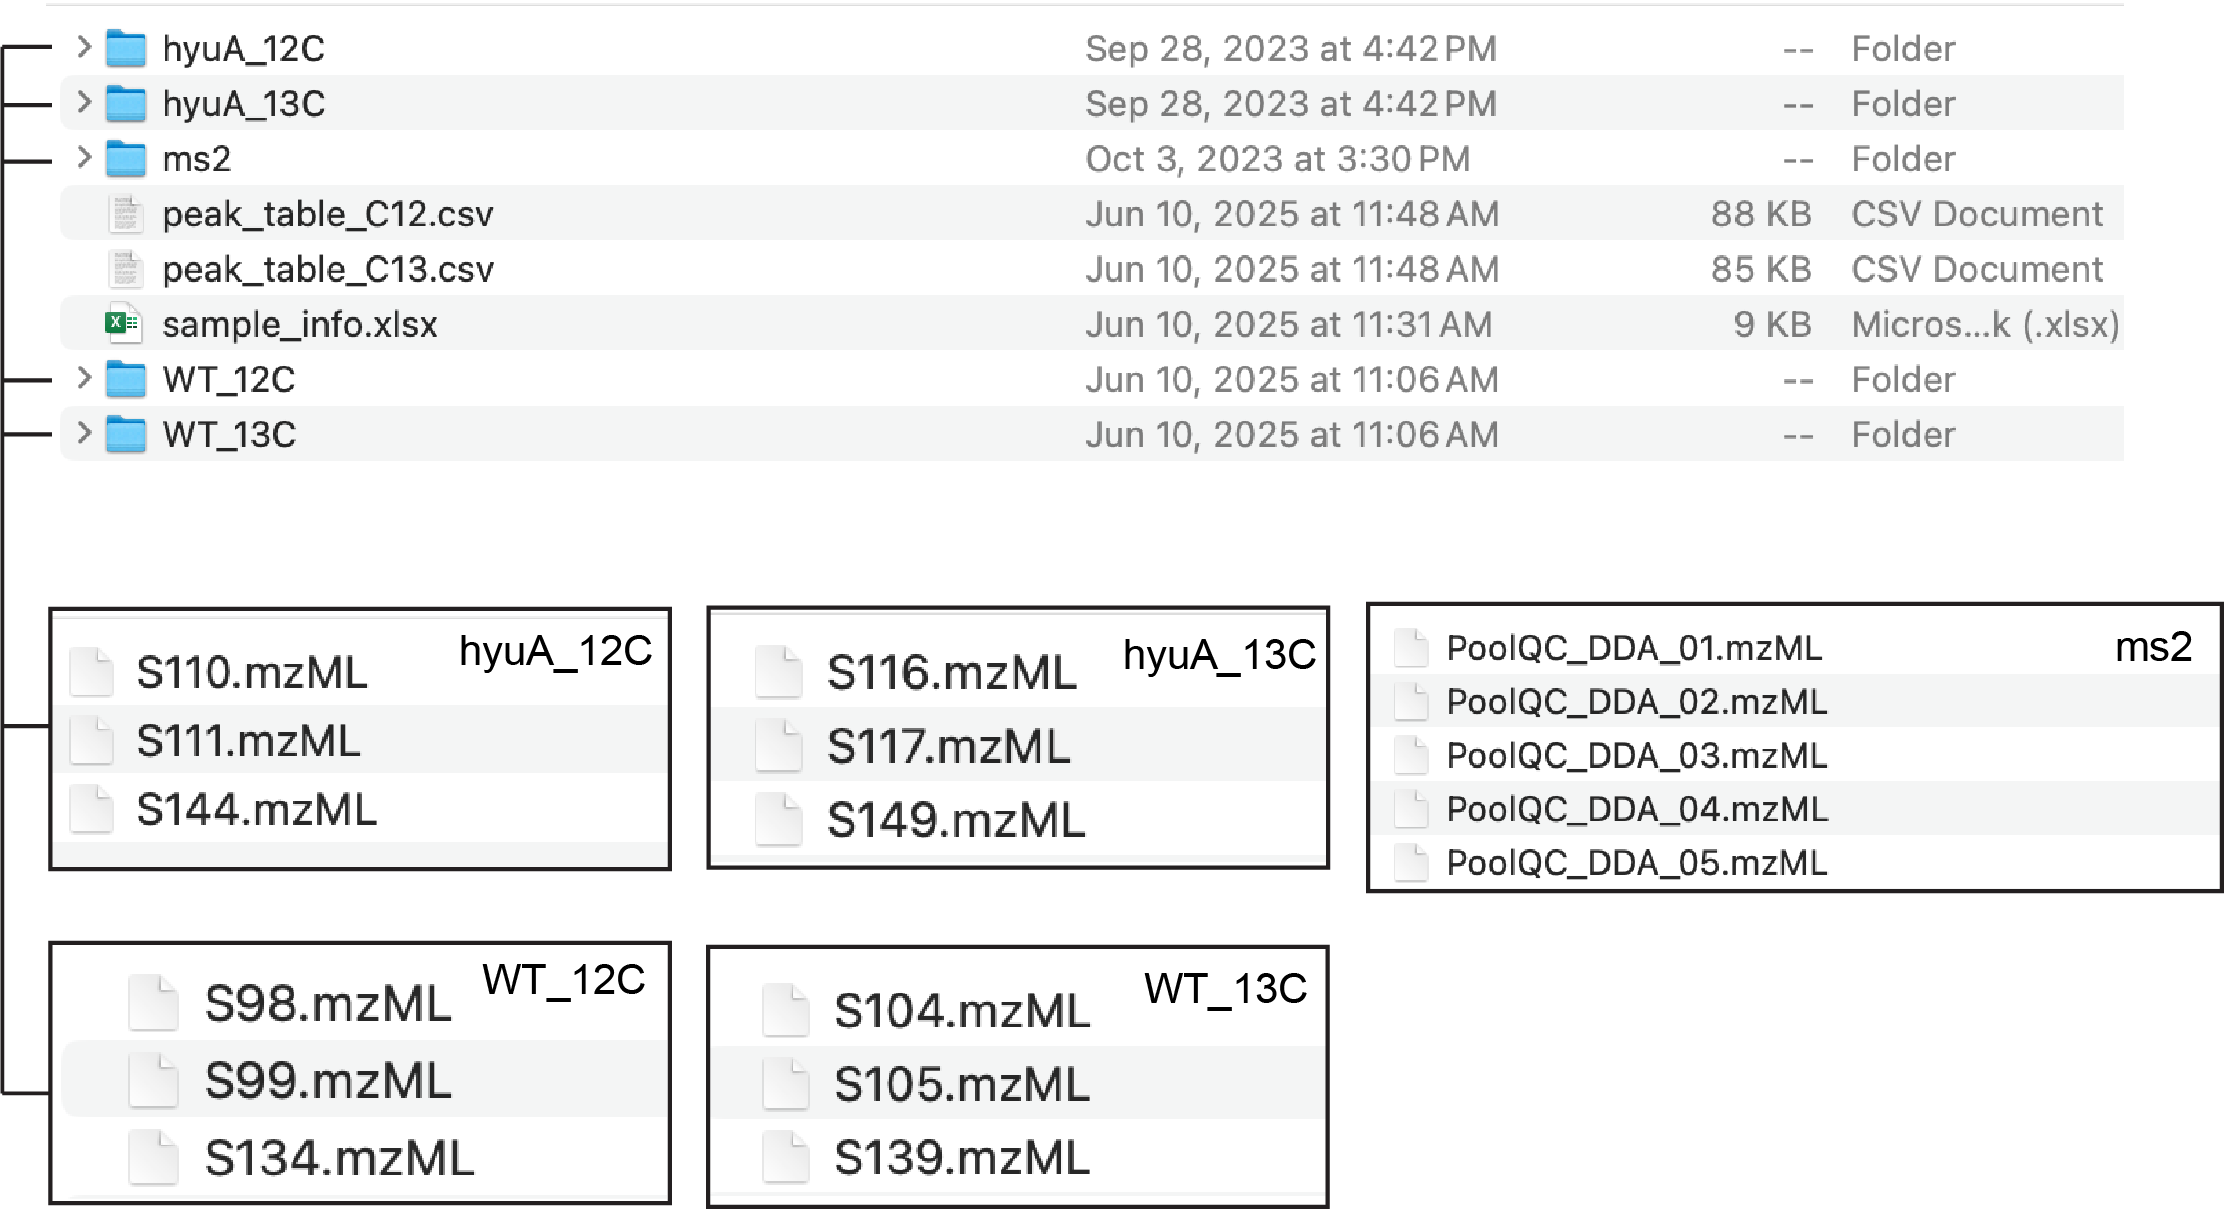
\includegraphics[keepaspectratio]{images/figure1_1.png}}

}

\caption{\label{fig-figure1-1}The screenshot of the demo data.}

\end{figure}%

\section{Run script}\label{run-script}

The basic use of IsoPairFinder is simply running the R script as below:

\begin{Shaded}
\begin{Highlighting}[]
\CommentTok{\# run the IsoPairFinder workflow}
\FunctionTok{library}\NormalTok{(tidyverse)}
\FunctionTok{library}\NormalTok{(IsoPairFinder)}

\CommentTok{\# analysis of HyuA }
\FunctionTok{find\_intemidates}\NormalTok{(}\AttributeTok{peak\_table\_unlabel =} \StringTok{\textquotesingle{}peak\_table\_C12.csv\textquotesingle{}}\NormalTok{,}
                 \AttributeTok{peak\_table\_label =} \StringTok{\textquotesingle{}peak\_table\_C13.csv\textquotesingle{}}\NormalTok{,}
                 \AttributeTok{sample\_info =} \StringTok{\textquotesingle{}sample\_info.xlsx\textquotesingle{}}\NormalTok{,}
                 \AttributeTok{path =} \StringTok{\textquotesingle{}\textasciitilde{}/Project/00\_Uric\_Acid\_project/Data/20250606\_isopairfind\_test/Demo\_data\_msdial/\textquotesingle{}}\NormalTok{,}
                 \AttributeTok{polarity =} \StringTok{\textquotesingle{}positive\textquotesingle{}}\NormalTok{,}
                 \AttributeTok{control\_group =} \FunctionTok{c}\NormalTok{(}\StringTok{"WT"}\NormalTok{),}
                 \AttributeTok{case\_group =} \FunctionTok{c}\NormalTok{(}\StringTok{\textquotesingle{}hyuA\textquotesingle{}}\NormalTok{),}
                 \AttributeTok{mz\_tol =} \DecValTok{10}\NormalTok{,}
                 \AttributeTok{rt\_tol =} \FloatTok{0.05}\NormalTok{,}
                 \AttributeTok{p\_value\_cutoff =} \FloatTok{0.05}\NormalTok{,}
                 \AttributeTok{p\_adjust =} \ConstantTok{TRUE}\NormalTok{,}
                 \AttributeTok{fold\_change\_cutoff =} \DecValTok{20}\NormalTok{,}
                 \AttributeTok{is\_recognize\_adducts =} \ConstantTok{TRUE}\NormalTok{)}
\end{Highlighting}
\end{Shaded}

Please refer to Section~\ref{sec-isoPairFinder-parameters} for the
explains of parameters.

\section{Output}\label{output}

After running, a new folder ``00\_tracer\_result'' will be created. It
contains several files, including ``tracer\_pair\_result.xlsx'' and
several PDF files. In the tab of the XLSX file, we could find the
identified ion pair results between the unlabeled and labeled groups
(Figure~\ref{fig-figure1-2}). The detailed explanations of each file can
be found in Section~\ref{sec-isoPairFinder-output}.

\begin{figure}

\centering{

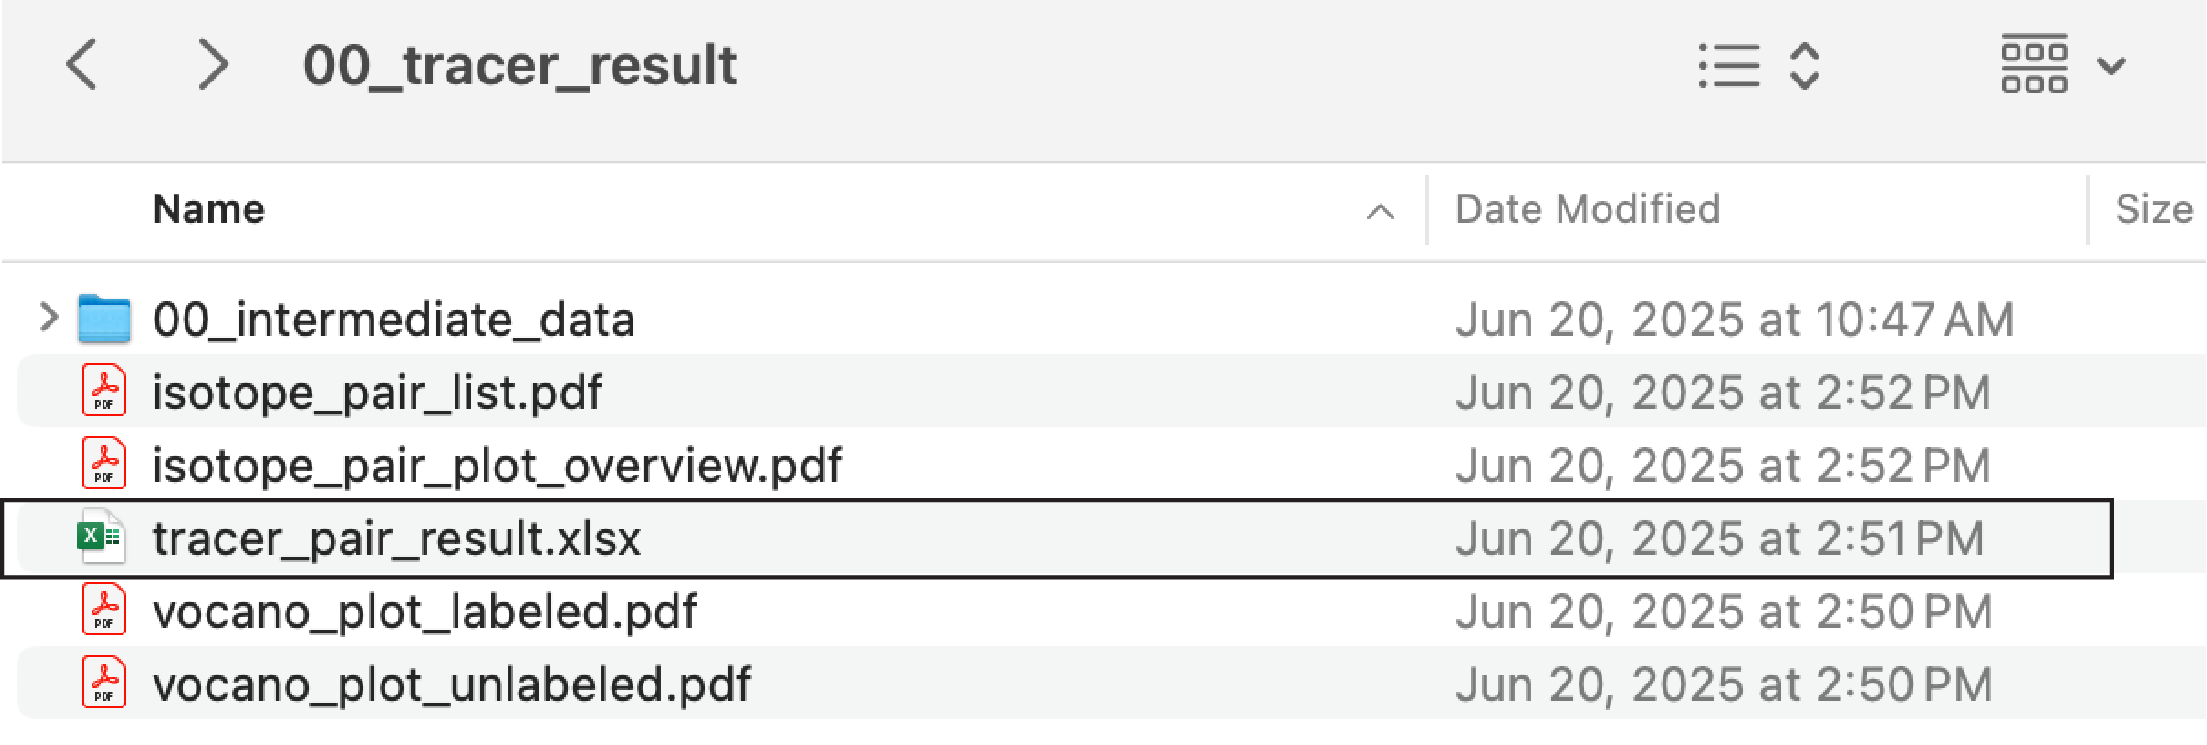
\includegraphics[width=0.75\linewidth,height=\textheight,keepaspectratio]{images/figure1_2.png}

}

\caption{\label{fig-figure1-2}Overview of results.}

\end{figure}%

\bookmarksetup{startatroot}

\chapter{Data Preparation}\label{sec-data-preparation}

The IsoPairFinder is designed to analyze stable isotope tracing
metabolomics data to identify the possible substrate candidates. Such a
study design needs: (i) an unlabeled group: mutant vs.~wild-type
cultures, (ii) a labeled group: mutant vs.~wild-type cultures.

For the input of IsoPairFinder, it needs two feature tables
(``peak\_table\_C12.csv'' and ``peak\_table\_C13.csv'') for each group,
and a table of sample information (``sample\_info.csv''). In addition,
the raw MS data files (in mzML or mzXML format) are needed and provided
in the folders. The demo data can be downloaded
\href{https://github.com/DoddLab/IsoPairFinder_demo_data}{here}.

Generally, it needs several files (Figure~\ref{fig-figure2-1}):

\begin{itemize}
\tightlist
\item
  \textbf{peak\_table\_C12.csv}: the peak area table of the unlabeled
  group (WT and HyuA mutants fed with uric acid).

  \begin{itemize}
  \tightlist
  \item
    The first 4 columns should be ``id'', ``mz'', ``rt'',
    ``ms1\_isotopes'', and other columns are sample names.
  \end{itemize}
\item
  \textbf{peak\_table\_C13.csv}: the peak area table of the labeled
  group (WT and HyuA mutants fed with 13C-uric acid).

  \begin{itemize}
  \tightlist
  \item
    The first 4 columns should be ``id'', ``mz'', ``rt'',
    ``ms1\_isotopes'', and other columns are sample names.
  \end{itemize}
\item
  \textbf{sample\_info.csv}: the sample information file in CSV/XLSX
  format.

  \begin{itemize}
  \tightlist
  \item
    The first 4 columns should be ``sample\_id'', ``group'',
    ``tracer\_group'', and ``type''.
  \item
    The ``sample\_id'' should be consistent with the sample names in the
    peak table.
  \item
    The ``group'' is the sample group. It only supports 2 groups in the
    IsoPairFinder version.
  \item
    The ``tracer\_group'' is the used tracers; it should be ``12C'' and
    ``13C''.
  \item
    The ``type'' is the sample type, e.g., ``sample'', ``qc'',
    ``blank''. Default: ``sample''
  \end{itemize}
\item
  \textbf{raw data (unlabeled \& control group)}: the folder contains
  raw data of the unlabeled WT.

  \begin{itemize}
  \tightlist
  \item
    The folder needed to be named as ``group\_tracer'', e.g.,
    ``WT\_12C''.
  \item
    It supports mzML/mzXML data format.
  \end{itemize}
\item
  \textbf{raw data (unlabeled \& case group)}: the folder contains raw
  data of unlabeled mutation (mzML).

  \begin{itemize}
  \tightlist
  \item
    The folder needed to be named as ``group\_tracer'', e.g.,
    ``hyuA\_12C''.
  \item
    It supports mzML/mzXML data format.
  \end{itemize}
\item
  \textbf{raw data (labeled \& control group)}: the folder contains raw
  data of labeled WT (mzML).

  \begin{itemize}
  \tightlist
  \item
    The folder needed to be named as ``group\_tracer'', e.g.,
    ``WT\_13C''.
  \item
    It supports mzML/mzXML data format.
  \end{itemize}
\item
  \textbf{raw data (labeled \& case group)}: the folder contains raw
  data of labeled mutation (mzML).

  \begin{itemize}
  \tightlist
  \item
    The folder needed to be named as ``group\_tracer'', e.g.,
    ``hyuA\_13C''.
  \item
    It supports mzML/mzXML data format.
  \end{itemize}
\item
  \textbf{ms2}: The folder includes MS/MS files (mzML/mzXML/mgf format)
\end{itemize}

\begin{figure}

\centering{

\pandocbounded{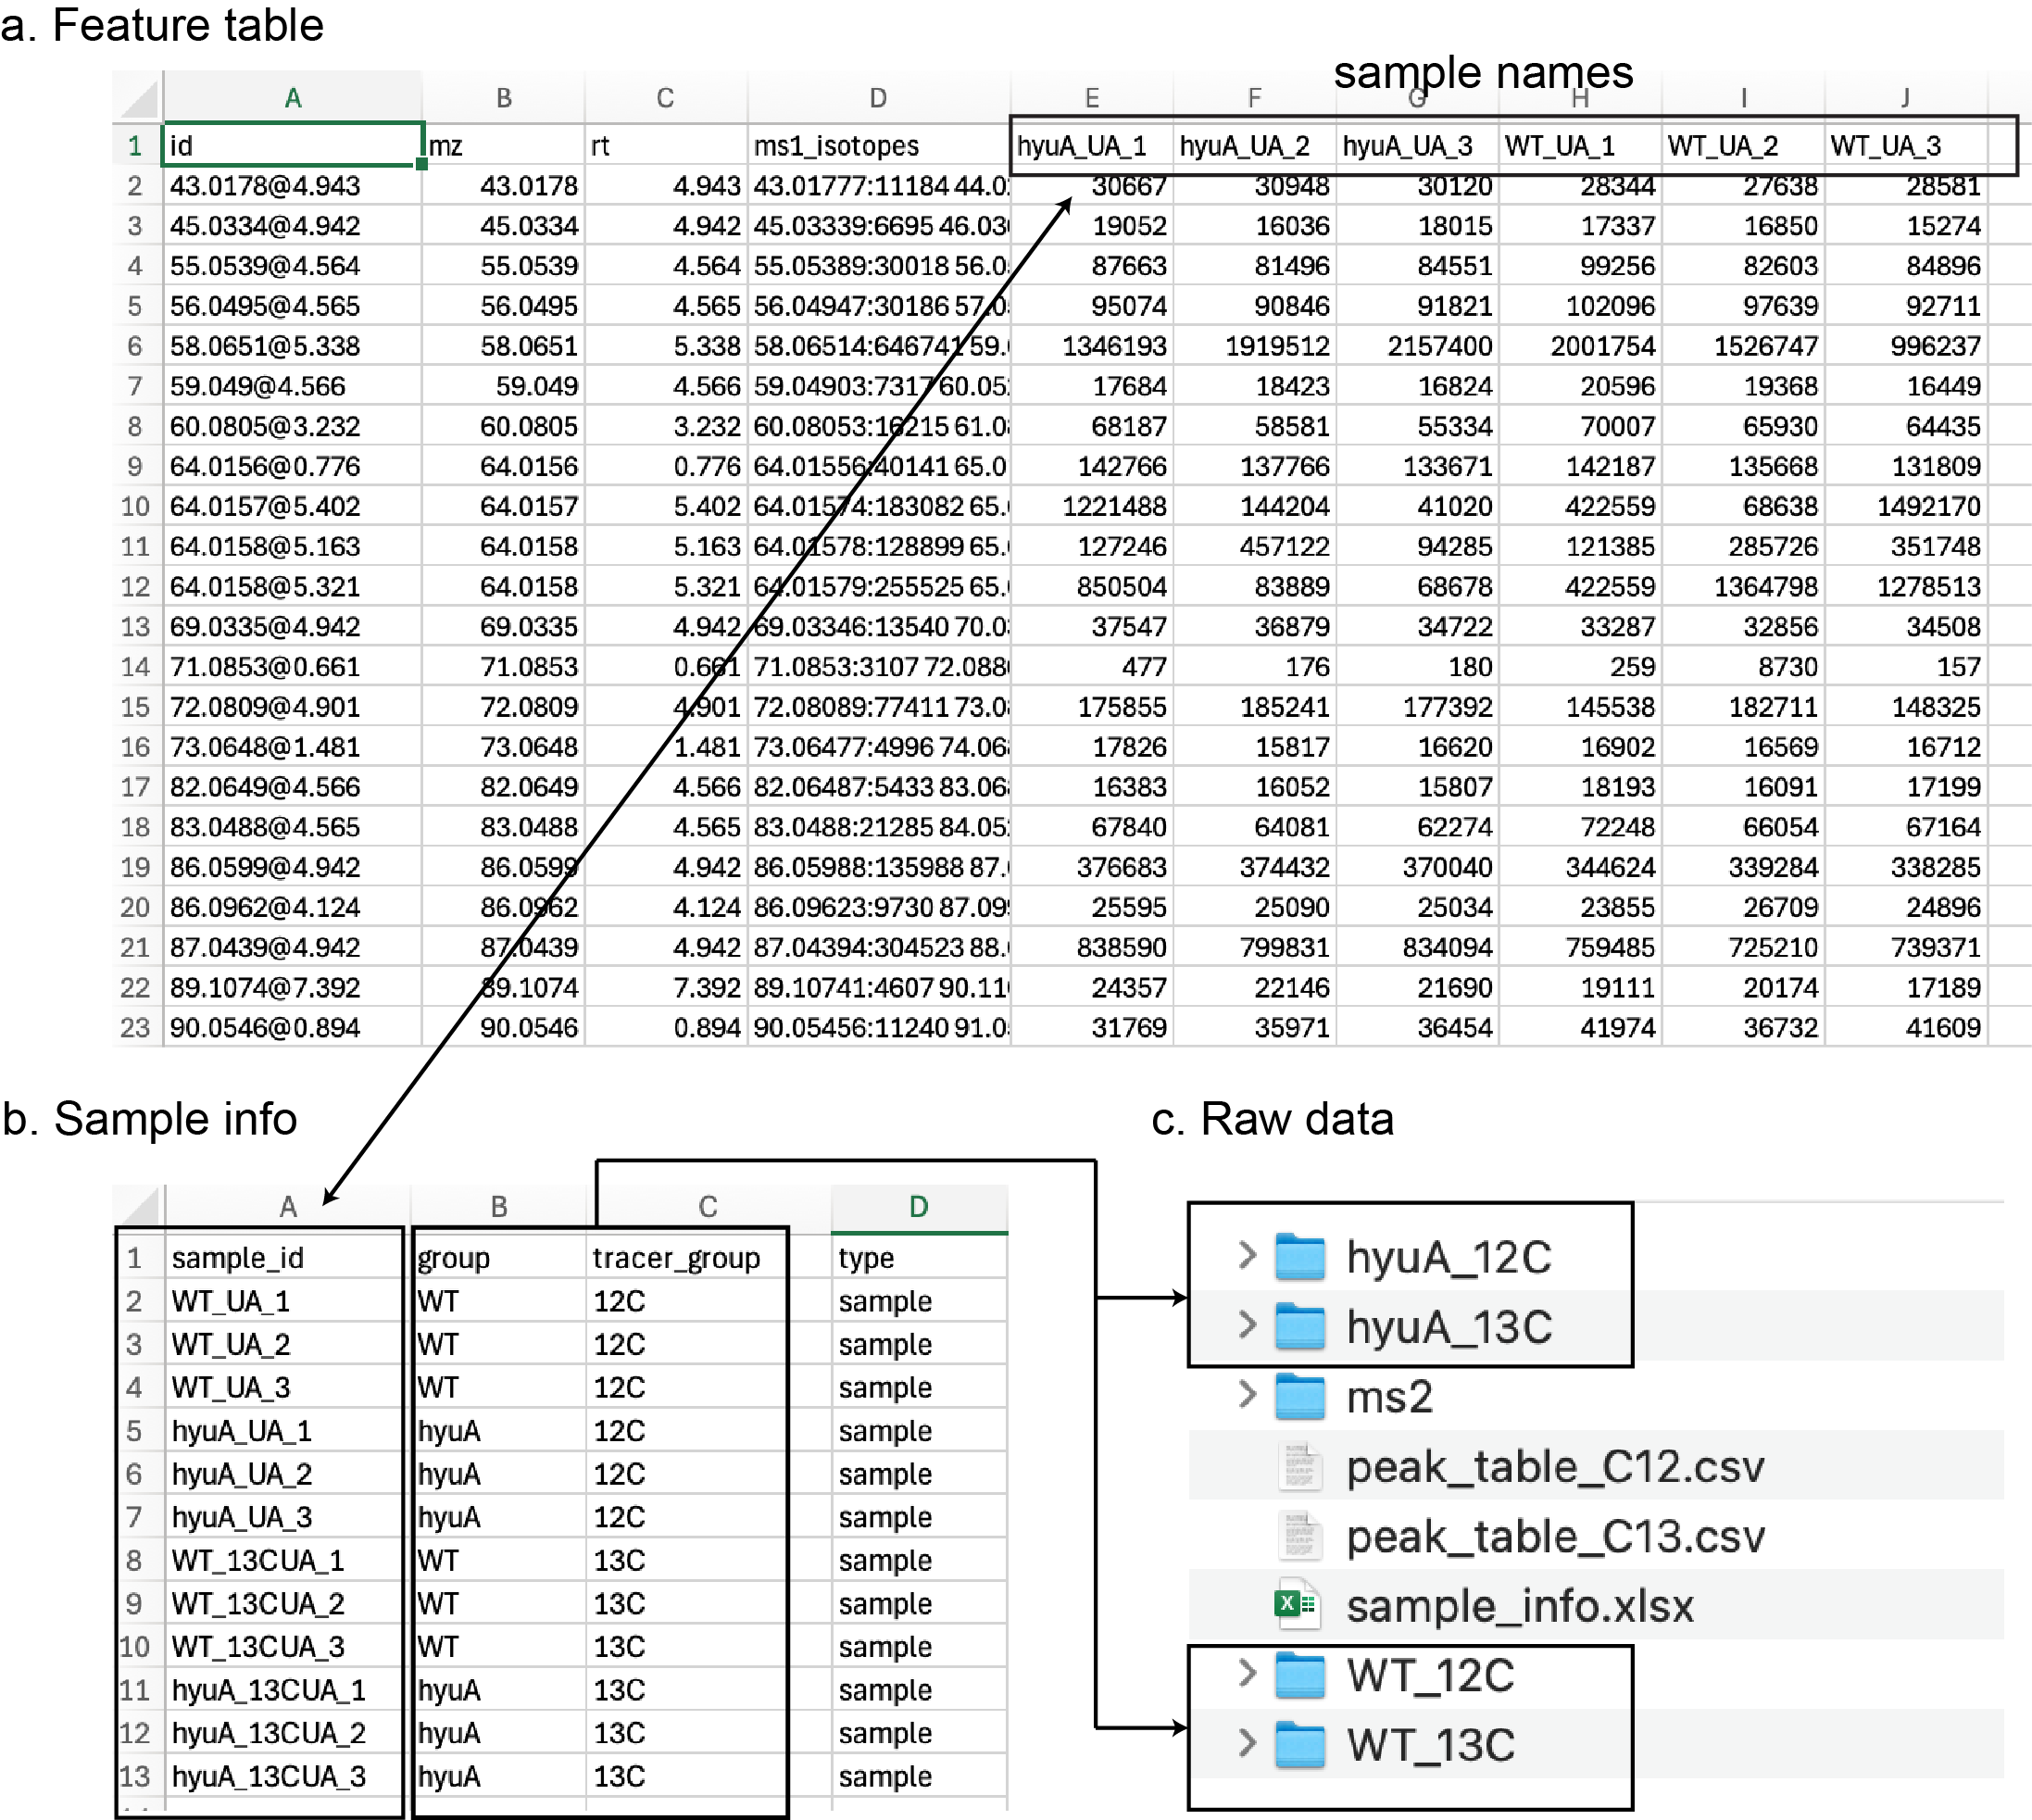
\includegraphics[keepaspectratio]{images/figure2_1.png}}

}

\caption{\label{fig-figure2-1}Input data files and format requirements.}

\end{figure}%

All input data files can be exported by different metabolomics data
processing tools, e.g.~xcms\textsuperscript{2},
MS-DIAL\textsuperscript{3}, and MZmine\textsuperscript{4}.
Table~\ref{tbl-table2-1} summarizes the links to demo data, processed
data, and tutorials of different tools. We provided step-by-step
instructions in the following parts. The raw data files were acquired
from the UHPLC-Agilent 6545XT QTOF. The study design could be found in
Chapter~\ref{sec-case-study}.

\begin{longtable}[]{@{}
  >{\raggedright\arraybackslash}p{(\linewidth - 8\tabcolsep) * \real{0.1897}}
  >{\raggedright\arraybackslash}p{(\linewidth - 8\tabcolsep) * \real{0.1897}}
  >{\raggedright\arraybackslash}p{(\linewidth - 8\tabcolsep) * \real{0.2759}}
  >{\raggedright\arraybackslash}p{(\linewidth - 8\tabcolsep) * \real{0.1724}}
  >{\raggedright\arraybackslash}p{(\linewidth - 8\tabcolsep) * \real{0.1724}}@{}}
\caption{Summary of demo data, processed results, and
tutorial}\label{tbl-table2-1}\tabularnewline
\toprule\noalign{}
\begin{minipage}[b]{\linewidth}\raggedright
Tool
\end{minipage} & \begin{minipage}[b]{\linewidth}\raggedright
Demo data
\end{minipage} & \begin{minipage}[b]{\linewidth}\raggedright
Processed data
\end{minipage} & \begin{minipage}[b]{\linewidth}\raggedright
Tutorial
\end{minipage} & \begin{minipage}[b]{\linewidth}\raggedright
section
\end{minipage} \\
\midrule\noalign{}
\endfirsthead
\toprule\noalign{}
\begin{minipage}[b]{\linewidth}\raggedright
Tool
\end{minipage} & \begin{minipage}[b]{\linewidth}\raggedright
Demo data
\end{minipage} & \begin{minipage}[b]{\linewidth}\raggedright
Processed data
\end{minipage} & \begin{minipage}[b]{\linewidth}\raggedright
Tutorial
\end{minipage} & \begin{minipage}[b]{\linewidth}\raggedright
section
\end{minipage} \\
\midrule\noalign{}
\endhead
\bottomrule\noalign{}
\endlastfoot
xcms\textsuperscript{2} &
\href{https://github.com/DoddLab/IsoPairFinder_DemoData_DiffTools/tree/main/00_raw_data}{Download}
&
\href{https://github.com/DoddLab/IsoPairFinder_DemoData_DiffTools/tree/main/01_input_data_IsoPairFinder/xcms}{Download}
&
\href{https://www.bioconductor.org/packages/release/bioc/html/xcms.html}{Tutorial}
& Section~\ref{sec-xcms} \\
MS-DIAL\textsuperscript{3} &
\href{https://github.com/DoddLab/IsoPairFinder_DemoData_DiffTools/tree/main/00_raw_data}{Download}
&
\href{https://github.com/DoddLab/IsoPairFinder_DemoData_DiffTools/tree/main/01_input_data_IsoPairFinder/msdial}{Download}
&
\href{https://systemsomicslab.github.io/mtbinfo.github.io/MS-DIAL/tutorial.html}{Tutorial}
& Section~\ref{sec-msdial} \\
MZmine\textsuperscript{4} &
\href{https://github.com/DoddLab/IsoPairFinder_DemoData_DiffTools/tree/main/00_raw_data}{Download}
&
\href{https://github.com/DoddLab/IsoPairFinder_DemoData_DiffTools/tree/main/01_input_data_IsoPairFinder/mzmine}{Download}
&
\href{https://mzmine.github.io/mzmine_documentation/index.html}{Tutorial}
& Section~\ref{sec-mzmine} \\
\end{longtable}

\section{xcms}\label{sec-xcms}

\subsection{Step 1: MS1 and MS2 data
conversion}\label{sec-xcms-conversion}

The raw data for the demo could be downloaded
\href{https://github.com/DoddLab/IsoPairFinder_DemoData_DiffTools/tree/main/00_raw_data}{here}.
Convert raw MS1 data and MS2 data files to mzML format using
ProteoWizard (version 3.0.23010,
\href{https://proteowizard.sourceforge.io/}{Link}). Please follow the
conversion settings (Figure~\ref{fig-figure2-2}).

\begin{figure}

\centering{

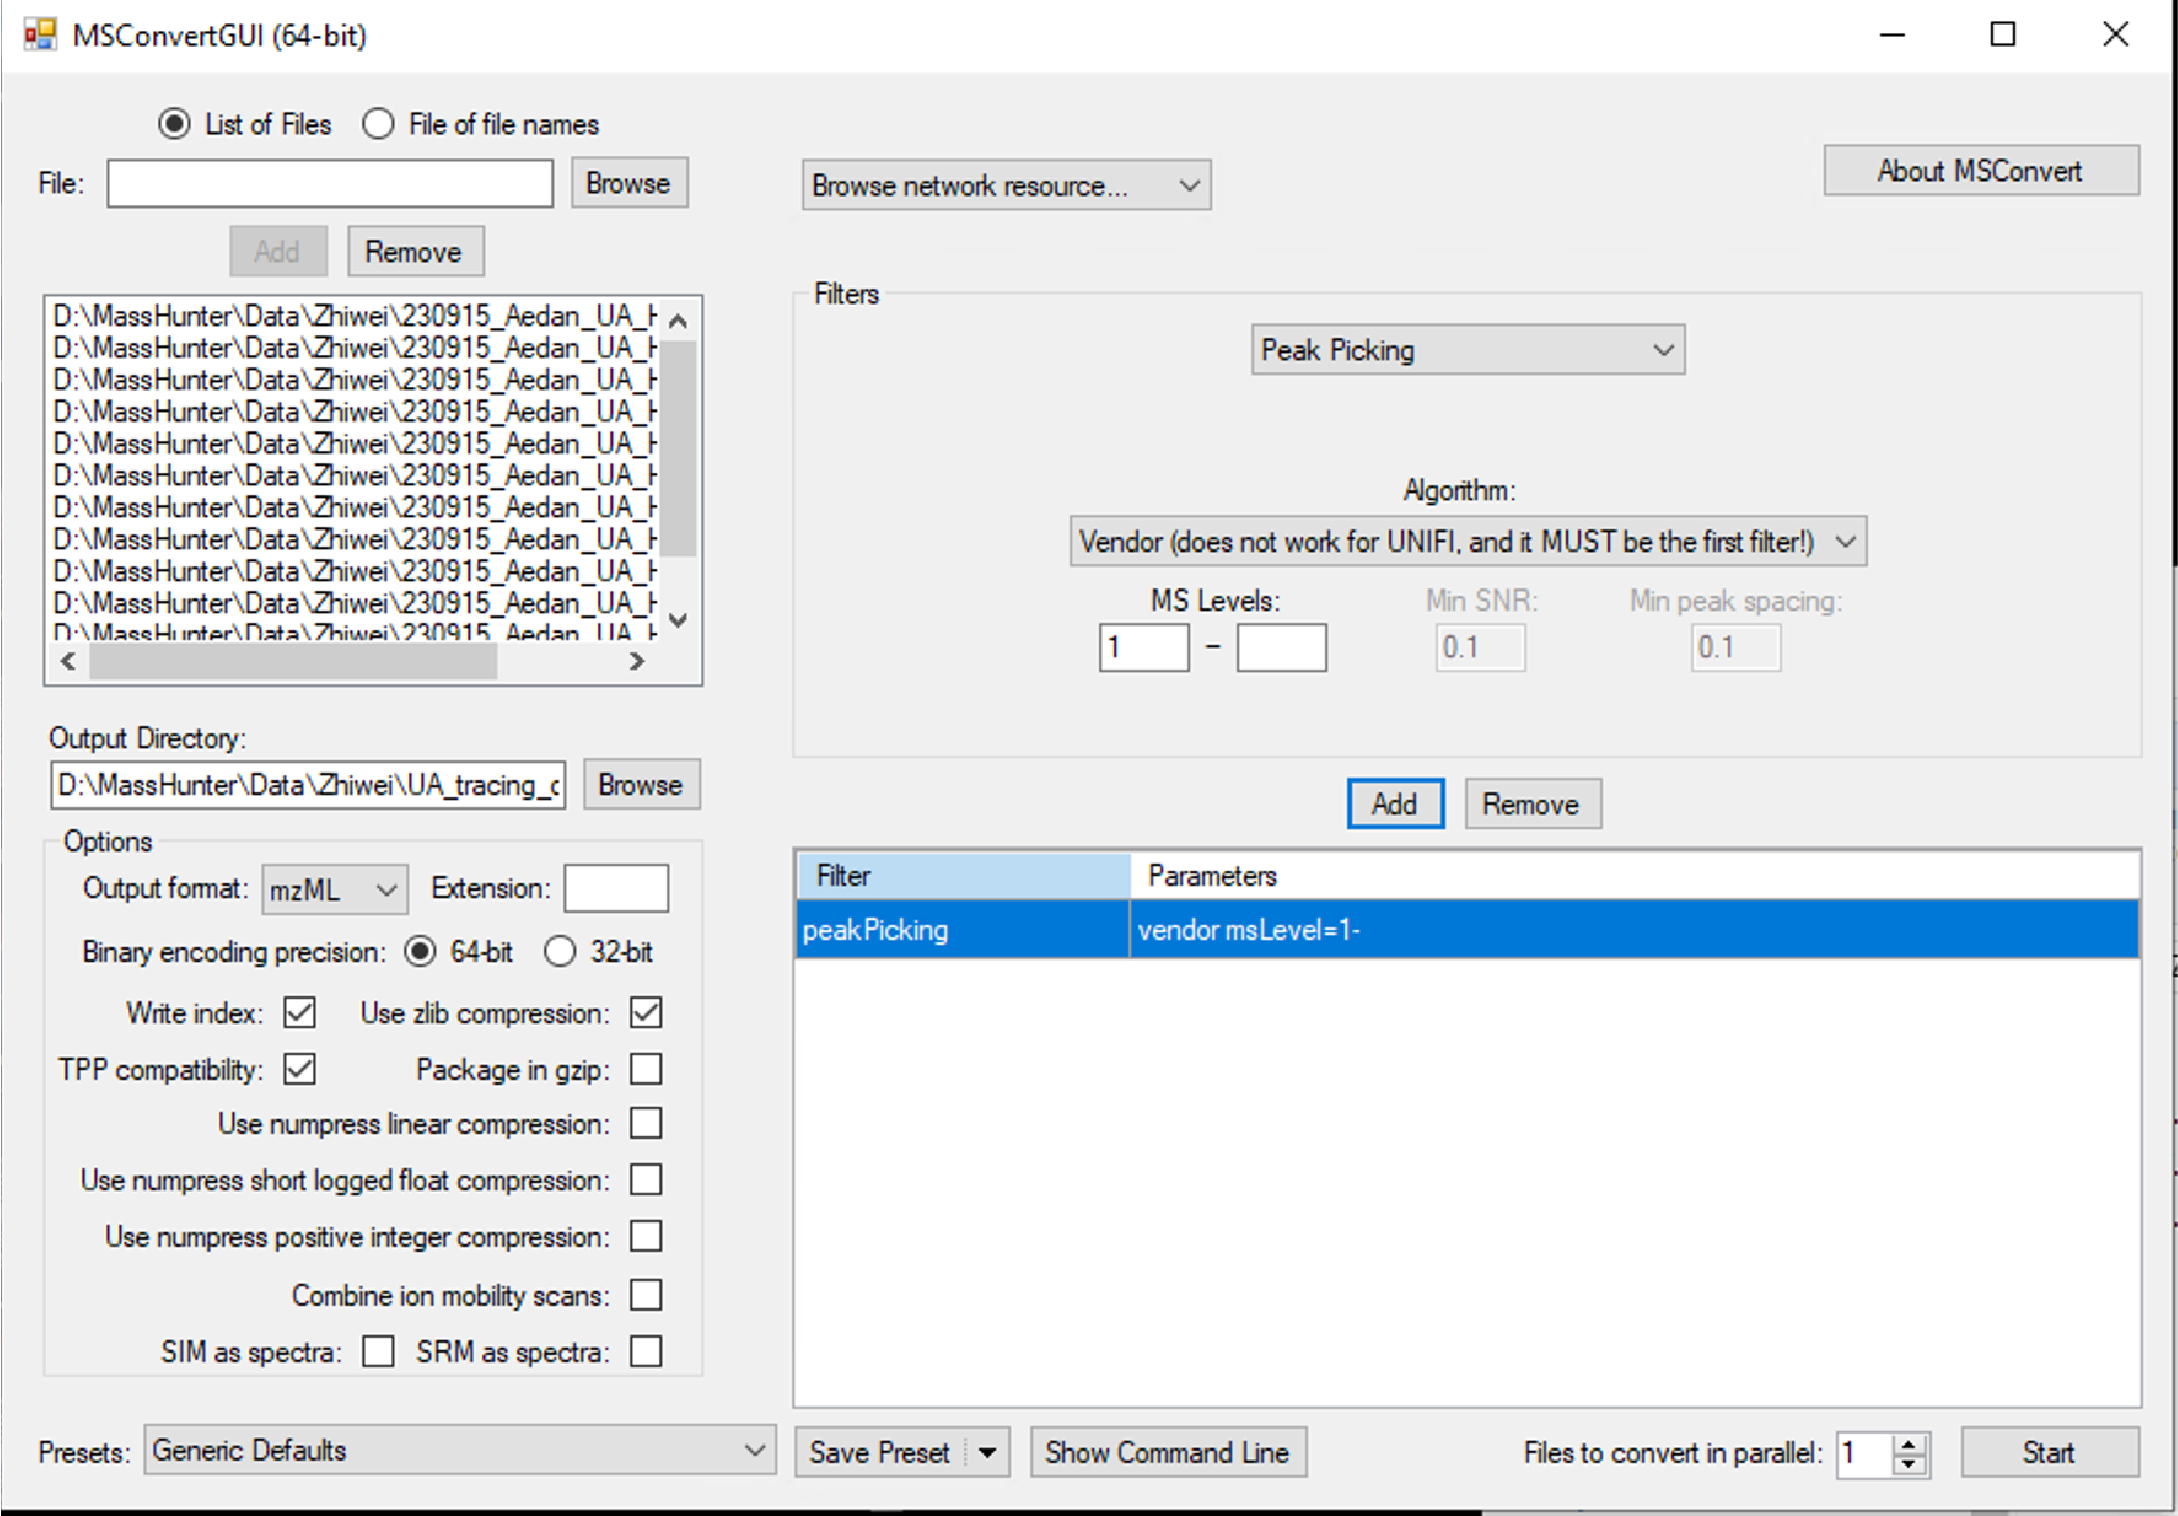
\includegraphics[width=0.75\linewidth,height=\textheight,keepaspectratio]{images/figure2_2.png}

}

\caption{\label{fig-figure2-2}ProteoWizard conversion settings.}

\end{figure}%

\subsection{Step 2. Peak picking using XCMS and isotope
merging}\label{step-2.-peak-picking-using-xcms-and-isotope-merging}

The R package \texttt{xcms} (version 3.20.0)\textsuperscript{2} for peak
detection and alignment, and the R package \texttt{CAMERA} (version
1.54.0)\textsuperscript{5} were used for isotope annotation.
\textbf{Note: The unlabeled group data and the labeled group data were
processed separately.}

\begin{itemize}
\tightlist
\item
  \textbf{Unlabeled group data processing}. The mzML files are placed in
  two folders named ``WT'' and ``hyuA\_12C'' according to their groups.
  These data were further processed with the following script.
\item
  \textbf{Labeled group data processing}. The mzML files are placed in
  two folders named ``WT'' and ``hyuA\_12C'' according to their groups.
  These data were further processed with the following script.
\end{itemize}

\begin{Shaded}
\begin{Highlighting}[]
\CommentTok{\# Load required packages}
\FunctionTok{library}\NormalTok{(xcms)}
\FunctionTok{library}\NormalTok{(CAMERA)}

\CommentTok{\# set the working path}
\FunctionTok{setwd}\NormalTok{(}\StringTok{\textquotesingle{}\textasciitilde{}/Project/00\_Uric\_Acid\_project/Data/20250606\_isopairfind\_test/Demo\_data\_xcms/00\_raw\_data\_processing\_12C/\textquotesingle{}}\NormalTok{)}

\CommentTok{\# DoddLabRawMS is a package which utilized xcms to process the raw data}
\NormalTok{devtools}\SpecialCharTok{::}\FunctionTok{install\_github}\NormalTok{(}\StringTok{\textquotesingle{}DoddLab/DoddLabRawMS\textquotesingle{}}\NormalTok{, }\AttributeTok{force =} \ConstantTok{TRUE}\NormalTok{)}

\CommentTok{\# load required packages}
\FunctionTok{library}\NormalTok{(tidyverse)}
\FunctionTok{library}\NormalTok{(xcms)}
\FunctionTok{library}\NormalTok{(CAMERA)}
\FunctionTok{library}\NormalTok{(DoddLabRawMS)}

\CommentTok{\# run raw data processing {-} 12C {-} unlabeled group}
\CommentTok{\# load parameter set}
\NormalTok{parameter\_set }\OtherTok{\textless{}{-}} \FunctionTok{initialize\_raw\_parameter\_class}\NormalTok{(}\AttributeTok{column =} \StringTok{\textquotesingle{}hilic\textquotesingle{}}\NormalTok{)}

\FunctionTok{process\_raw\_data}\NormalTok{(}\AttributeTok{parameter\_set =}\NormalTok{ parameter\_set, }
                 \AttributeTok{path =} \StringTok{\textquotesingle{}\textasciitilde{}/Project/00\_Uric\_Acid\_project/Data/20250606\_isopairfind\_test/Demo\_data\_xcms/00\_raw\_data\_processing\_12C/\textquotesingle{}}\NormalTok{)}


\CommentTok{\# run CAMERA to annotate the isotopes}
\FunctionTok{load}\NormalTok{(}\StringTok{\textquotesingle{}\textasciitilde{}/Project/00\_Uric\_Acid\_project/Data/20250606\_isopairfind\_test/Demo\_data\_xcms/00\_raw\_data\_processing\_12C/00\_raw\_data\_processing/00\_intermediate\_data/xset3.RData\textquotesingle{}}\NormalTok{)}
\NormalTok{path }\OtherTok{\textless{}{-}} \StringTok{\textquotesingle{}\textasciitilde{}/Project/00\_Uric\_Acid\_project/Data/20250606\_isopairfind\_test/Demo\_data\_xcms/00\_raw\_data\_processing\_12C/\textquotesingle{}}

\FunctionTok{runCAMERA}\NormalTok{(}\AttributeTok{xset =}\NormalTok{ xset3,}
          \AttributeTok{path =}\NormalTok{ path,}
          \AttributeTok{polarity =} \StringTok{\textquotesingle{}positive\textquotesingle{}}\NormalTok{,}
          \AttributeTok{nSlaves =} \DecValTok{6}\NormalTok{,}
          \AttributeTok{pg\_sigma =} \DecValTok{6}\NormalTok{,}
          \AttributeTok{pg\_perfwhm =} \FloatTok{0.6}\NormalTok{,}
          \AttributeTok{iso\_maxcharge =} \DecValTok{2}\NormalTok{,}
          \AttributeTok{iso\_maxiso =} \DecValTok{4}\NormalTok{,}
          \AttributeTok{iso\_ppm =} \DecValTok{25}\NormalTok{,}
          \AttributeTok{iso\_mzabs =} \FloatTok{0.01}\NormalTok{,}
          \AttributeTok{iso\_minfrac =} \FloatTok{0.5}\NormalTok{,}
          \AttributeTok{is\_vali\_pg\_cor =} \ConstantTok{FALSE}\NormalTok{,}
          \AttributeTok{pg\_cor\_eic\_th =} \FloatTok{0.7}\NormalTok{,}
          \AttributeTok{pg\_cor\_calcIso =} \ConstantTok{FALSE}\NormalTok{,}
          \AttributeTok{gp\_cor\_calcCis =} \ConstantTok{TRUE}\NormalTok{,}
          \AttributeTok{gp\_cor\_calcCaS =} \ConstantTok{FALSE}\NormalTok{,}
          \AttributeTok{gp\_cor\_cor\_exp\_th =} \FloatTok{0.75}\NormalTok{,}
          \AttributeTok{is\_use\_modified\_rule =} \ConstantTok{TRUE}\NormalTok{,}
          \AttributeTok{adduct\_ppm =} \DecValTok{25}\NormalTok{,}
          \AttributeTok{adduct\_mzabs =} \FloatTok{0.01}\NormalTok{)}
\end{Highlighting}
\end{Shaded}

\subsection{Step 3. Feature table
modification}\label{step-3.-feature-table-modification}

The xcms exported feature table could be quickly modified using the
IsoPairFinder functions \texttt{modify\_xcms\_table()}. The sample\_info
table (Figure~\ref{fig-figure2-1}) is needed to define the samples and
groups.

\begin{Shaded}
\begin{Highlighting}[]
\CommentTok{\# Load required packages}
\FunctionTok{library}\NormalTok{(IsoPairFinder)}
\FunctionTok{modify\_xcms\_table}\NormalTok{(}\AttributeTok{table\_xcms =} \StringTok{\textquotesingle{}\textasciitilde{}/Project/00\_Uric\_Acid\_project/Data/20250606\_isopairfind\_test/Demo\_data\_xcms/00\_raw\_data\_processing\_12C/00\_raw\_data\_processing/Peak{-}table.csv\textquotesingle{}}\NormalTok{,}
                  \AttributeTok{table\_camera =} \StringTok{\textquotesingle{}\textasciitilde{}/Project/00\_Uric\_Acid\_project/Data/20250606\_isopairfind\_test/Demo\_data\_xcms/00\_raw\_data\_processing\_12C/00\_raw\_data\_processing/adduct\_result\_camera.xlsx\textquotesingle{}}\NormalTok{,}
                  \AttributeTok{table\_sample\_info =} \StringTok{\textquotesingle{}\textasciitilde{}/Project/00\_Uric\_Acid\_project/Data/20250606\_isopairfind\_test/Demo\_data\_xcms/sample\_info.xlsx\textquotesingle{}}\NormalTok{,}
                  \AttributeTok{path =} \StringTok{\textquotesingle{}\textasciitilde{}/Project/00\_Uric\_Acid\_project/Data/20250606\_isopairfind\_test/Demo\_data\_xcms/00\_raw\_data\_processing\_12C\textquotesingle{}}\NormalTok{,}
                  \AttributeTok{file\_output =} \StringTok{\textquotesingle{}peak\_table\_C12.csv\textquotesingle{}}\NormalTok{)}
\end{Highlighting}
\end{Shaded}

\subsection{Step 4. Organizing files}\label{step-4.-organizing-files}

Please move the modified feature tables, the sample information table,
the MS2 data files, and the raw data files to the designated location
(Figure~\ref{fig-figure2-1}).

\section{MS-DIAL}\label{sec-msdial}

\subsection{Step 1: MS1 and MS2 data
conversion}\label{step-1-ms1-and-ms2-data-conversion}

The raw data for the demo could be downloaded
\href{https://github.com/DoddLab/IsoPairFinder_DemoData_DiffTools/tree/main/00_raw_data}{here}.
Convert raw MS1 data to ABF format using
\texttt{Analysis\ Base\ File\ Converter} (version 1.3.8802,
Figure~\ref{fig-figure2-3}).

\begin{figure}

\centering{

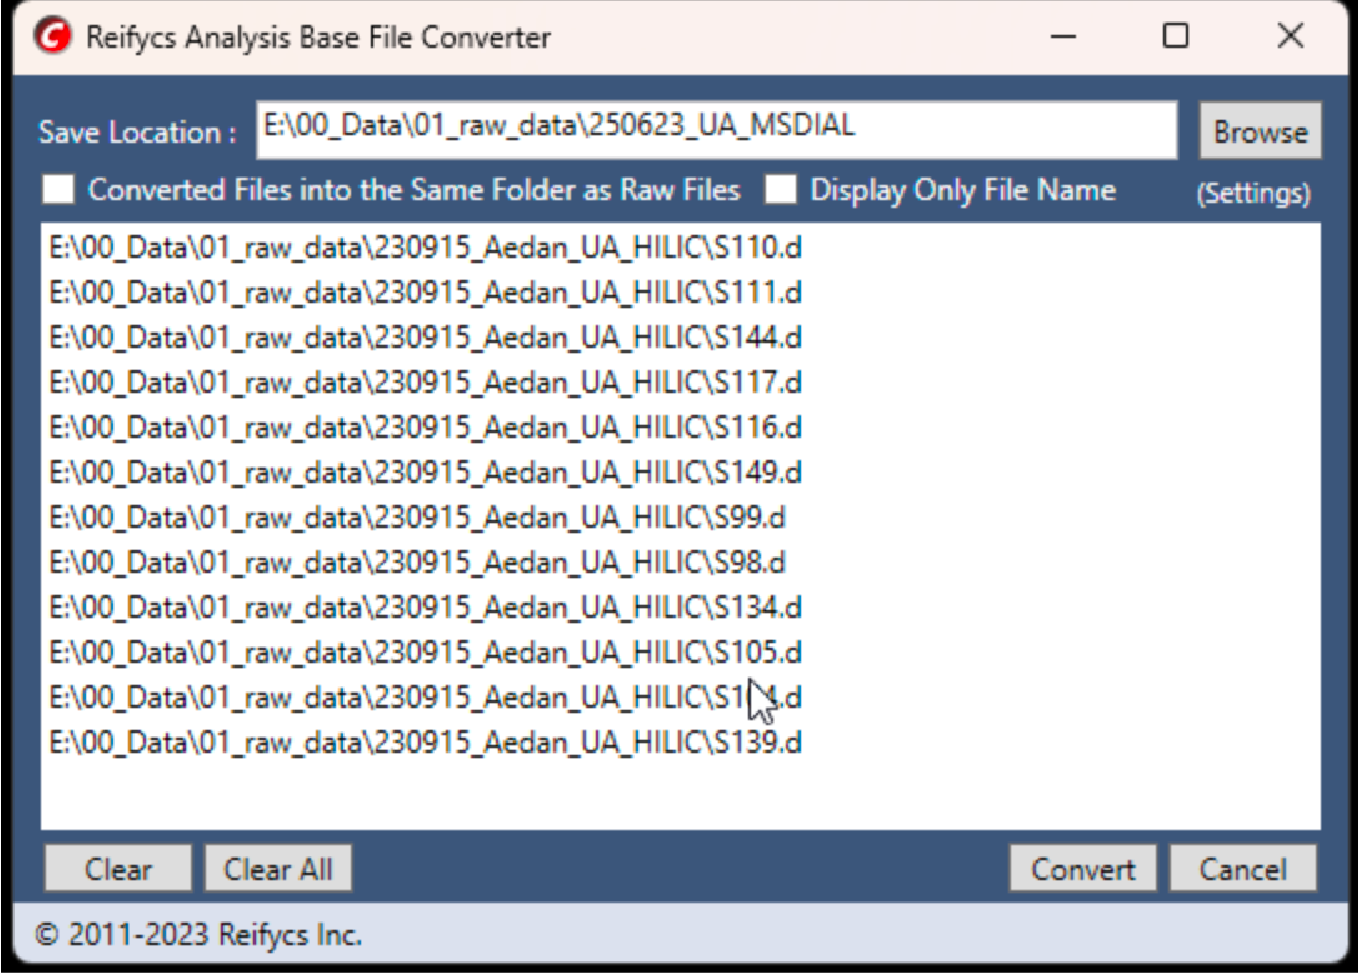
\includegraphics[width=0.75\linewidth,height=\textheight,keepaspectratio]{images/figure2_3.png}

}

\caption{\label{fig-figure2-3}ABF conversion settings.}

\end{figure}%

Convert MS2 data files to mzML format using ProteoWizard (version
3.0.23010, \href{https://proteowizard.sourceforge.io/}{Link}). The
parameters could be found in Figure~\ref{fig-figure2-2}.

\subsection{Step 2. Peak picking using
MS-DIAL}\label{step-2.-peak-picking-using-ms-dial}

The \texttt{MS-DIAL} (ver.4.9.221218) was used here. Select the
appropriate parameters according to the experimental design (parameters
used in the demo data are shown in Figure~\ref{fig-figure2-4}). Export
the feature table containing ``Raw data matrix (Area)''. \textbf{Note:
The unlabeled group data and the labeled group data were processed
separately.}

\begin{figure}

\centering{

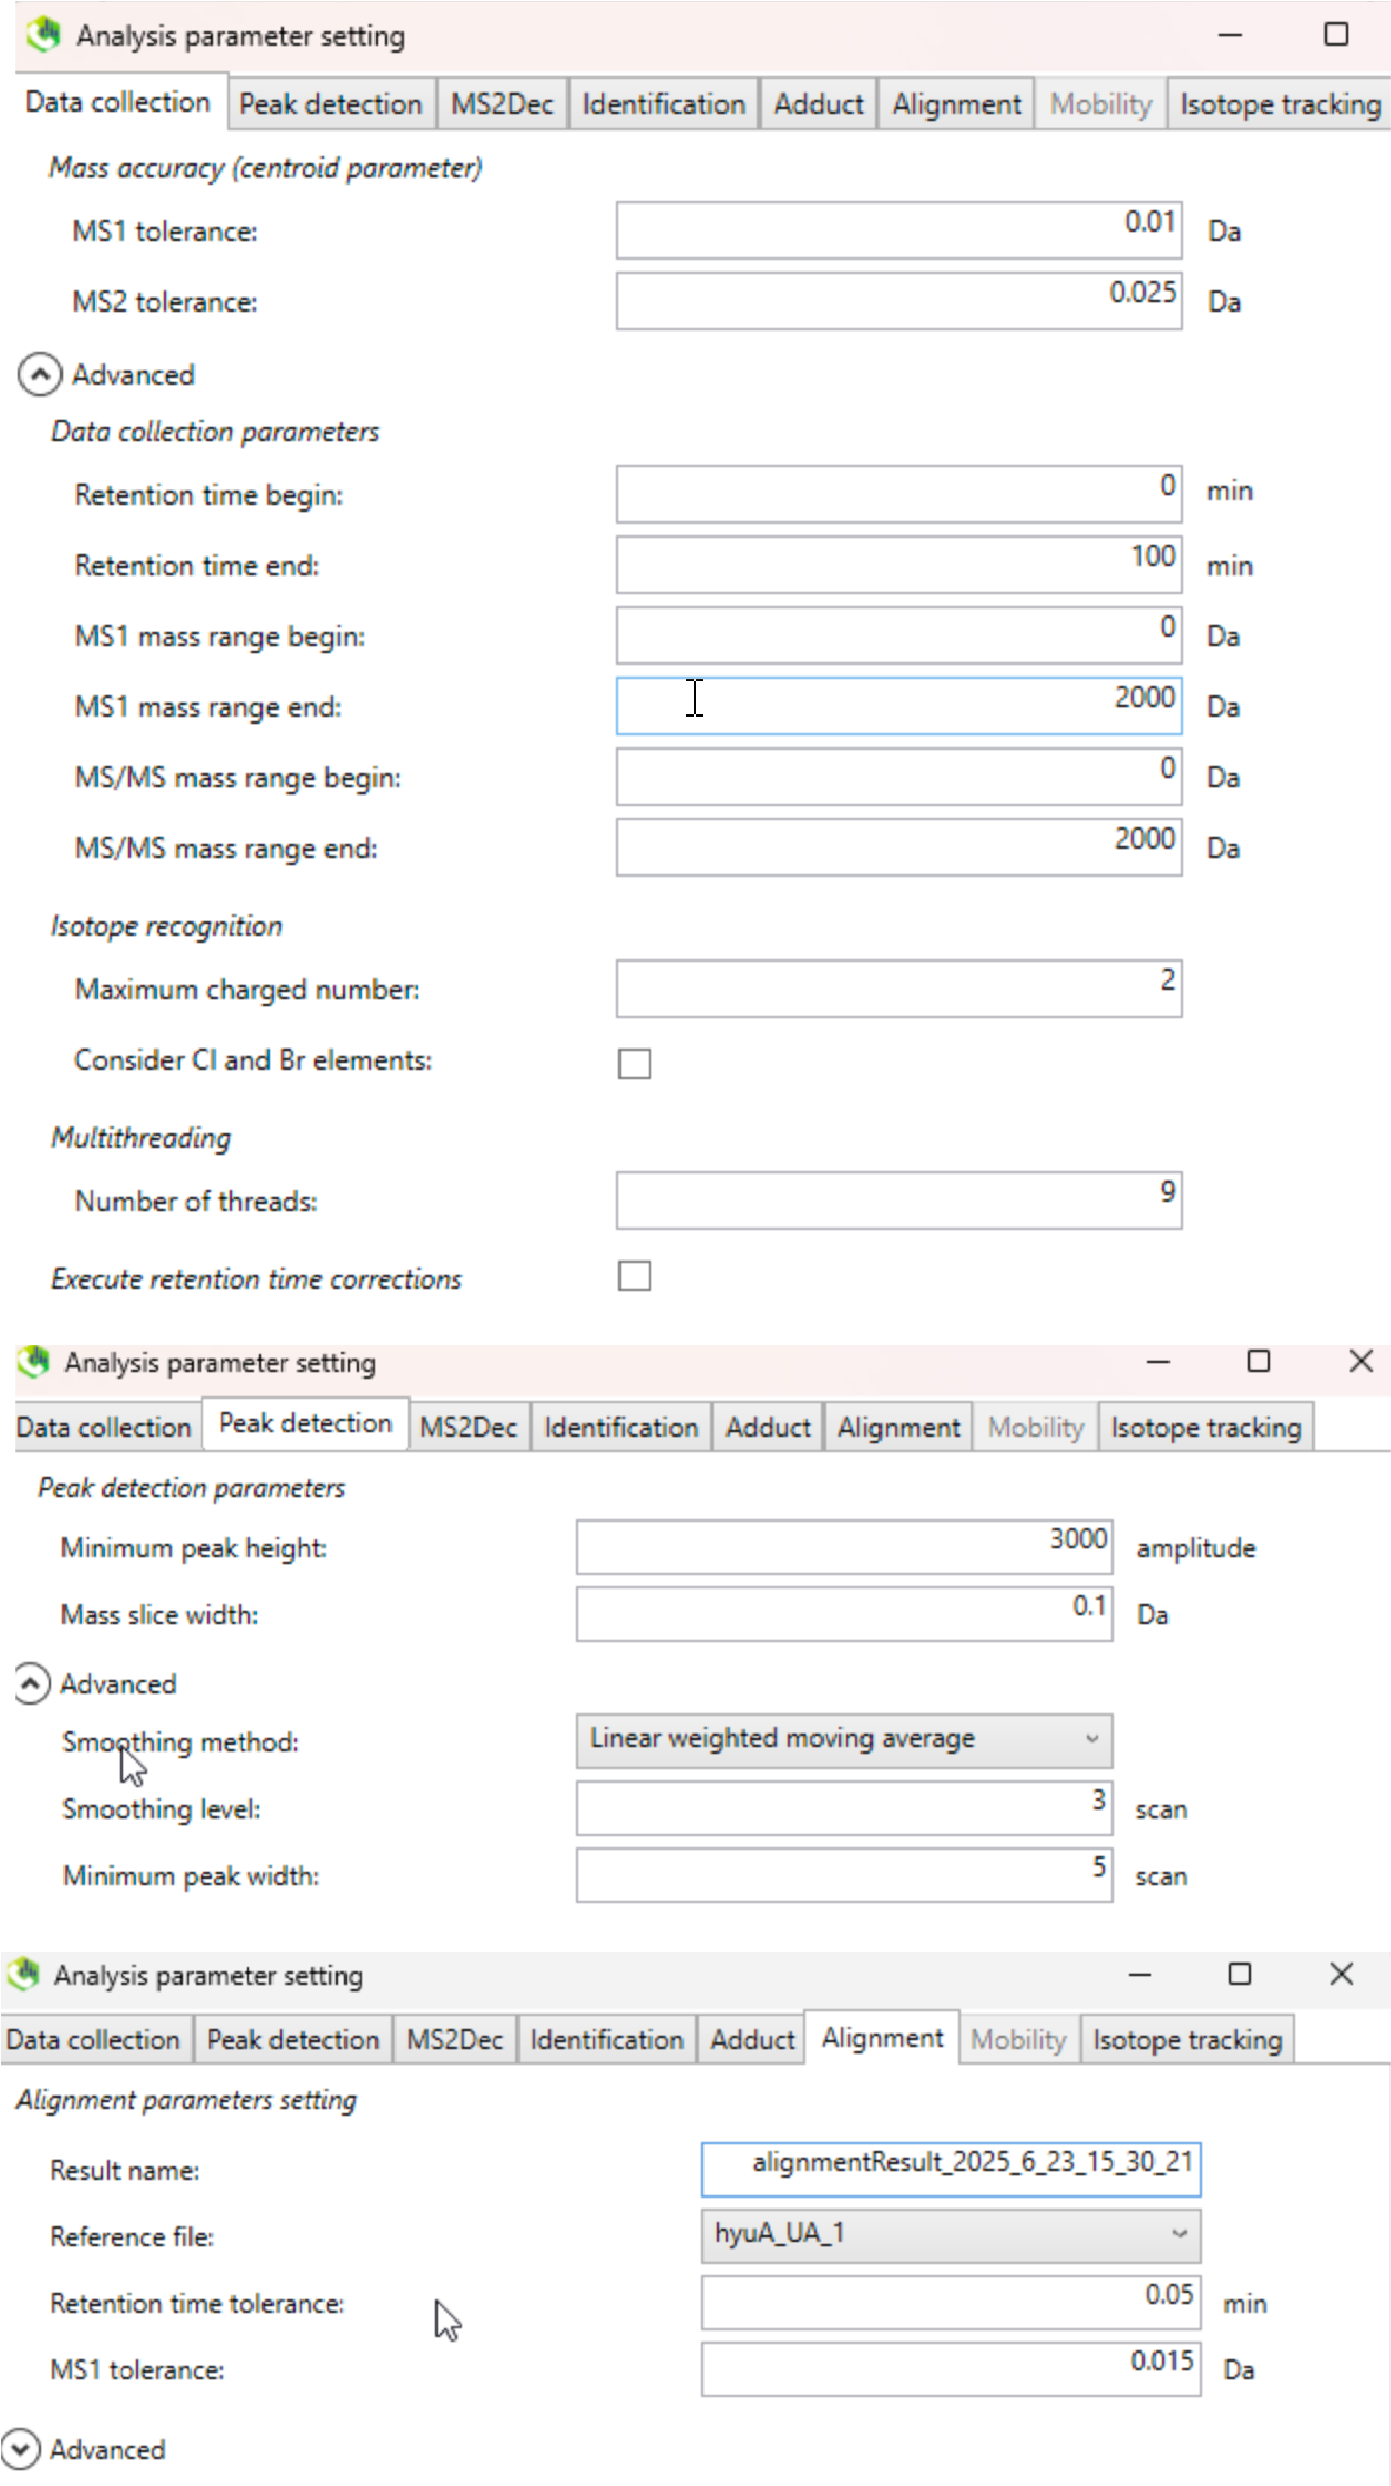
\includegraphics[width=0.5\linewidth,height=\textheight,keepaspectratio]{images/figure2_4.png}

}

\caption{\label{fig-figure2-4}MS-DIAL peak picking settings.}

\end{figure}%

\subsection{Step 3. Feature table
modification}\label{step-3.-feature-table-modification-1}

The MS-DIAL exported feature table could be quickly modified using the
IsoPairFinder functions \texttt{modify\_msdial\_table()}. The
sample\_info table (Figure~\ref{fig-figure2-1}) is needed to define the
samples and groups.

\begin{Shaded}
\begin{Highlighting}[]
\FunctionTok{library}\NormalTok{(IsoPairFinder)}
\NormalTok{table\_msdial }\OtherTok{\textless{}{-}} \StringTok{\textquotesingle{}\textasciitilde{}/Project/00\_Uric\_Acid\_project/Data/20250606\_isopairfind\_test/Demo\_data\_msdial/hyuA\_UA\_48h\_area.txt\textquotesingle{}}
\NormalTok{table\_sample\_info }\OtherTok{\textless{}{-}} \StringTok{\textquotesingle{}\textasciitilde{}/Project/00\_Uric\_Acid\_project/Data/20250606\_isopairfind\_test/Demo\_data\_msdial/sample\_info.xlsx\textquotesingle{}}

\FunctionTok{modify\_msdial\_table}\NormalTok{(}\AttributeTok{table\_msdial =}\NormalTok{ table\_msdial,}
                    \AttributeTok{table\_sample\_info =}\NormalTok{ table\_sample\_info,}
                    \AttributeTok{path =} \StringTok{\textquotesingle{}\textasciitilde{}/Project/00\_Uric\_Acid\_project/Data/20250606\_isopairfind\_test/Demo\_data\_msdial\textquotesingle{}}\NormalTok{,}
                    \AttributeTok{file\_output =} \StringTok{\textquotesingle{}peak\_table\_C12.csv\textquotesingle{}}\NormalTok{)}
\end{Highlighting}
\end{Shaded}

\subsection{Step 4. Organizing files}\label{step-4.-organizing-files-1}

Please move the modified feature tables, the sample information table,
the MS2 data files, and the raw data files to the designated location
(Figure~\ref{fig-figure2-1}).

\section{MZmine}\label{sec-mzmine}

\subsection{Step 1: MS1 and MS2 data
conversion}\label{step-1-ms1-and-ms2-data-conversion-1}

The raw data for the demo could be downloaded
\href{https://github.com/DoddLab/IsoPairFinder_DemoData_DiffTools/tree/main/00_raw_data}{here}.
Convert raw MS1 data and MS2 data files to mzML format using
ProteoWizard (version 3.0.23010,
\href{https://proteowizard.sourceforge.io/}{Link}; See
Section~\ref{sec-xcms-conversion}).

\subsection{Step 2. Peak picking using
MZmine}\label{step-2.-peak-picking-using-mzmine}

The \texttt{MZmine} (version 4.7.3) was used here. Import and load the
default parameters (the ``UHPLC-QTOF'' was used here). The modified
parameters used in the demo data are shown in
Figure~\ref{fig-figure2-5}. \textbf{Note: The unlabeled group data and
the labeled group data were processed separately.}

\begin{figure}

\centering{

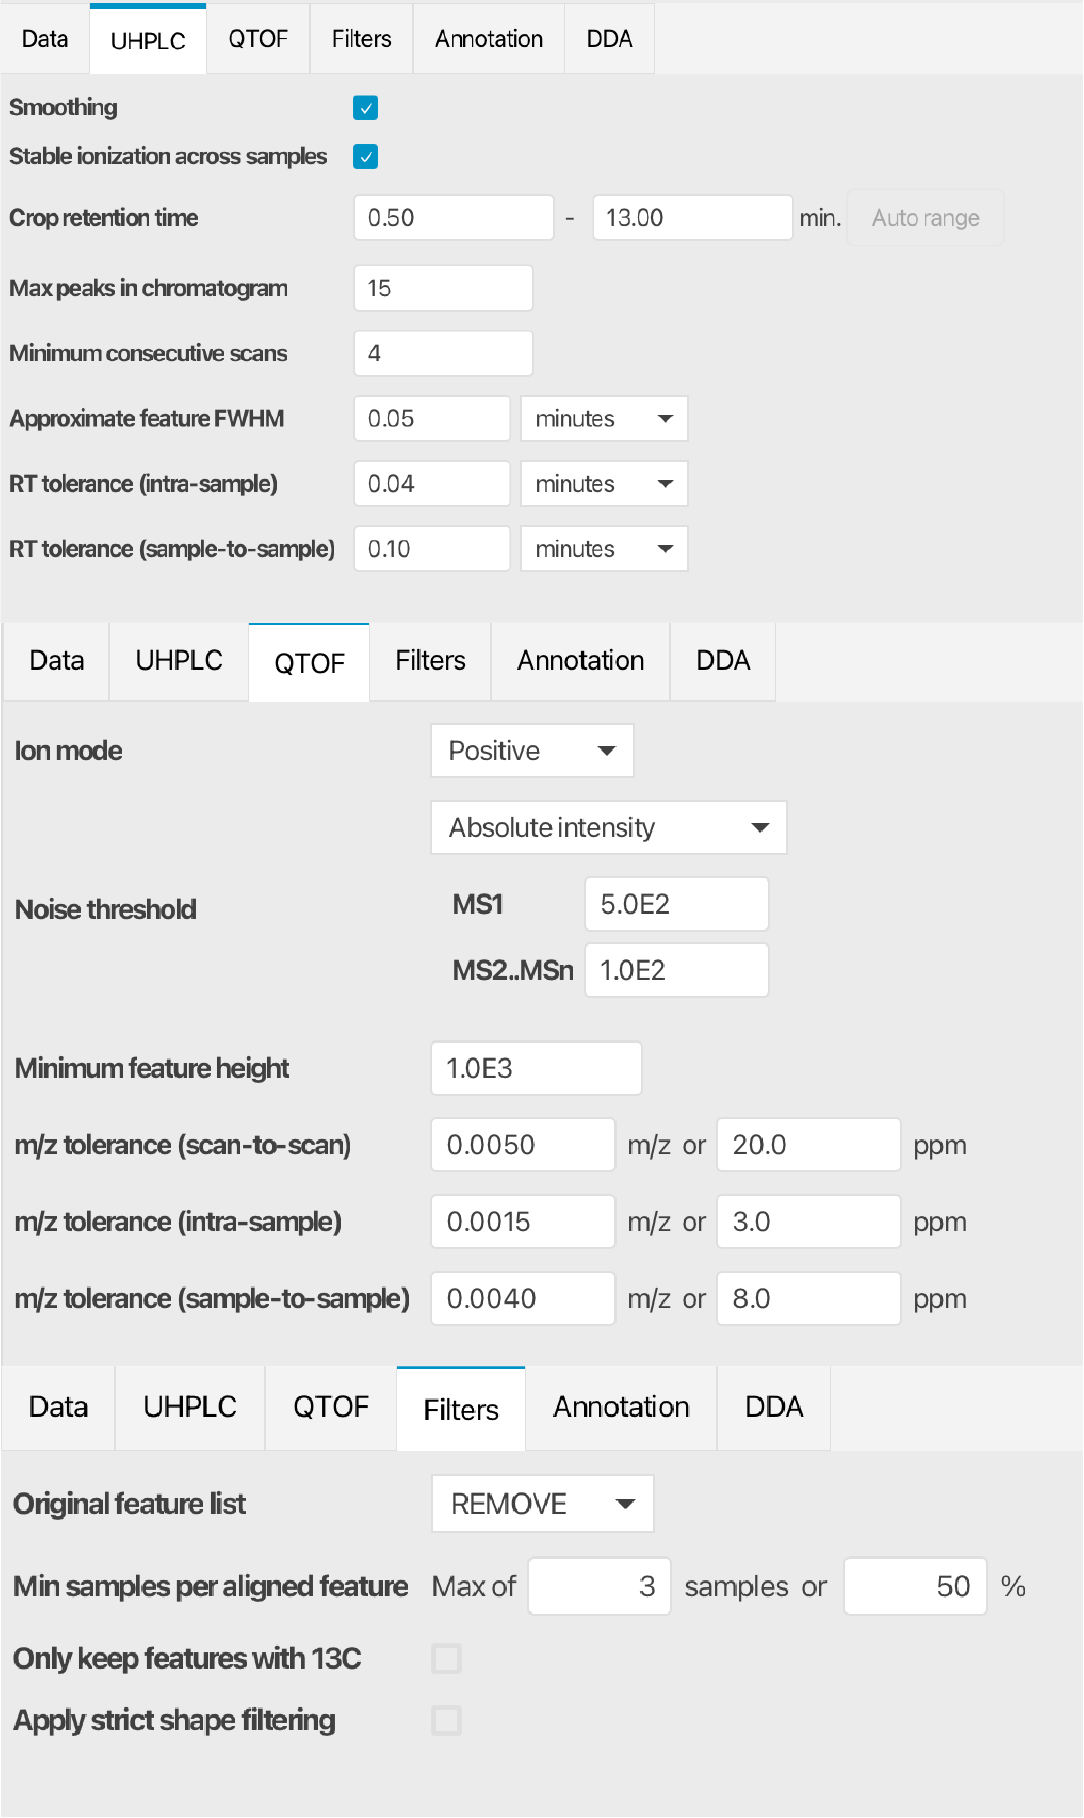
\includegraphics[width=0.75\linewidth,height=\textheight,keepaspectratio]{images/figure2_5.png}

}

\caption{\label{fig-figure2-5}MZmine peak picking settings.}

\end{figure}%

Export the feature table using MZmine:\\
\textbf{Feature list methods → Export feature list → Export CSV legacy
MZmine2} (see Figure~\ref{fig-figure2-6}).

\begin{figure}

\centering{

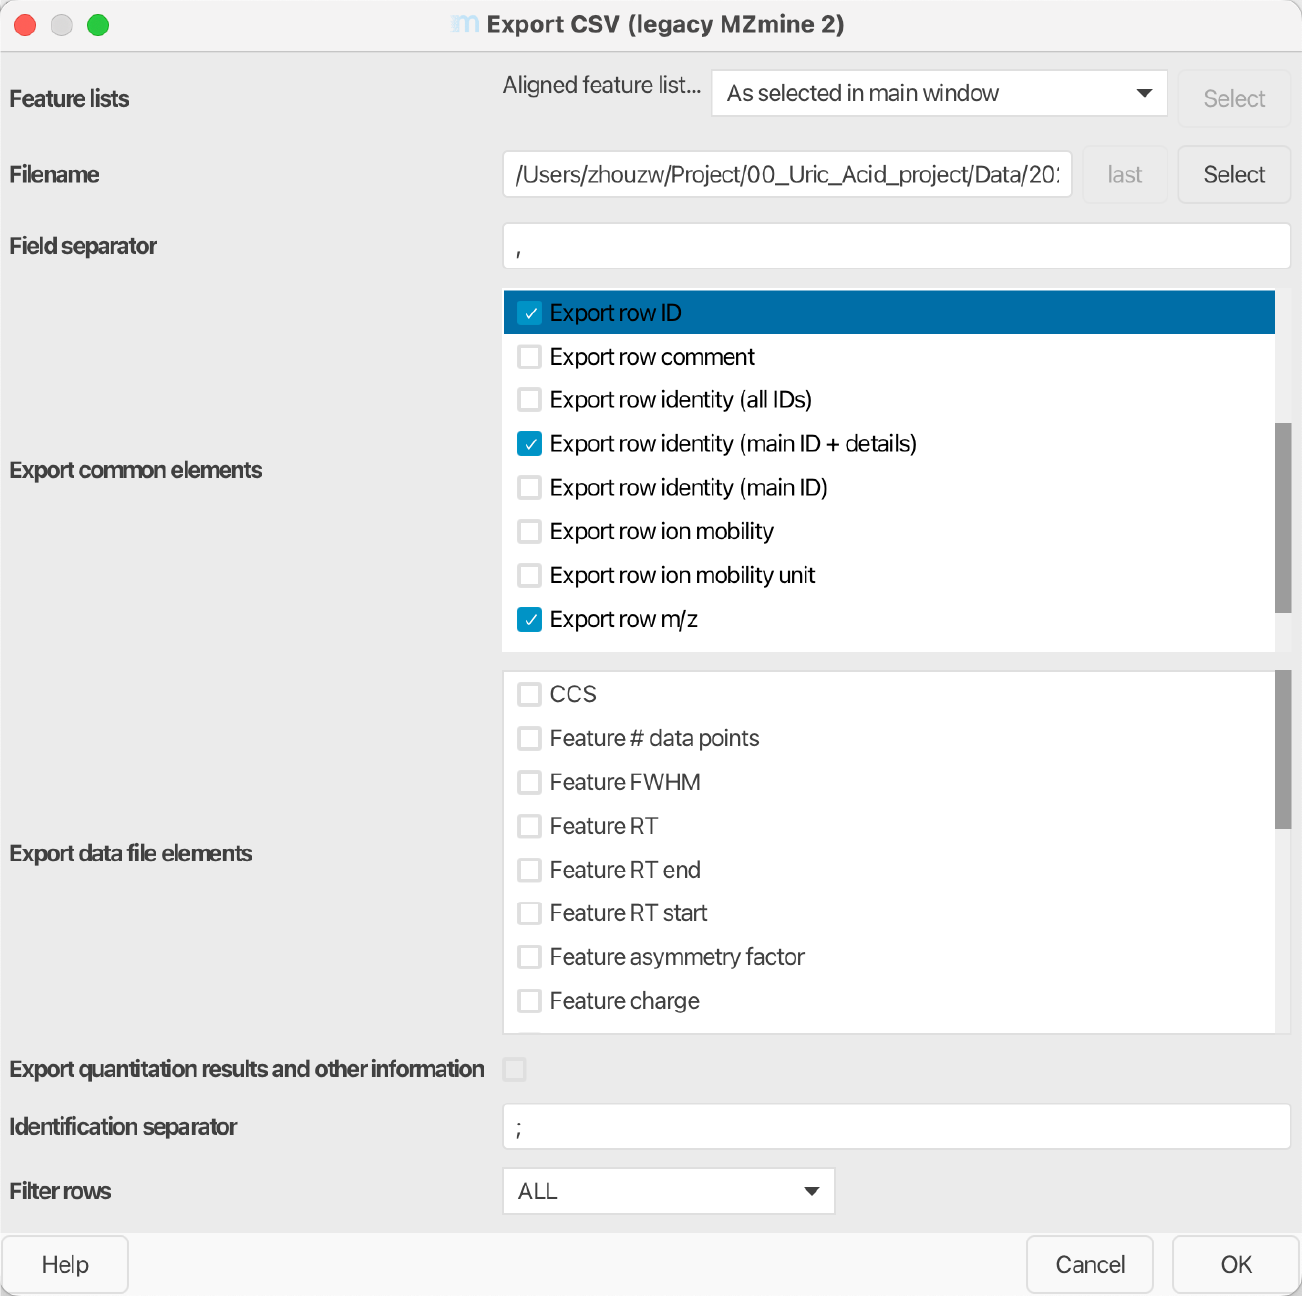
\includegraphics[width=0.75\linewidth,height=\textheight,keepaspectratio]{images/figure2_6.png}

}

\caption{\label{fig-figure2-6}MZmine feature table export settings.}

\end{figure}%

\subsection{Step 3. Feature table
modification}\label{step-3.-feature-table-modification-2}

The exported feature table can be quickly modified using the
IsoPairFinder function \texttt{modify\_mzmine\_table()}. The
sample\_info table (Figure~\ref{fig-figure2-1}) is needed to define the
samples and groups.

\begin{Shaded}
\begin{Highlighting}[]
\CommentTok{\# Load required packages}
\FunctionTok{library}\NormalTok{(IsoPairFinder)}
\NormalTok{table\_mzmine }\OtherTok{\textless{}{-}} \StringTok{\textquotesingle{}\textasciitilde{}/Project/00\_Uric\_Acid\_project/Data/20250606\_isopairfind\_test/Demo\_data\_mzmine/mzmine\_12C.csv\textquotesingle{}}
\NormalTok{table\_sample\_info }\OtherTok{\textless{}{-}} \StringTok{\textquotesingle{}\textasciitilde{}/Project/00\_Uric\_Acid\_project/Data/20250606\_isopairfind\_test/Demo\_data\_mzmine/sample\_info.xlsx\textquotesingle{}}
\FunctionTok{modify\_mzmine\_table}\NormalTok{(}\AttributeTok{table\_mzmine =}\NormalTok{ table\_mzmine,}
                    \AttributeTok{table\_sample\_info =}\NormalTok{ table\_sample\_info,}
                    \AttributeTok{path =} \StringTok{\textquotesingle{}\textasciitilde{}/Project/00\_Uric\_Acid\_project/Data/20250606\_isopairfind\_test/Demo\_data\_mzmine\textquotesingle{}}\NormalTok{,}
                    \AttributeTok{file\_output =} \StringTok{\textquotesingle{}peak\_table\_C12.csv\textquotesingle{}}\NormalTok{)}
\end{Highlighting}
\end{Shaded}

\subsection{Step 4. Organizing files}\label{step-4.-organizing-files-2}

Please move the modified feature tables, the sample information table,
the MS2 data files, and the raw data files to the designated location
(Figure~\ref{fig-figure2-1}).

\bookmarksetup{startatroot}

\chapter{IsoPairFinder running}\label{sec-isoPairFinder-running}

\section{Overview of the IsoPairFinder
workflow}\label{overview-of-the-isopairfinder-workflow}

Generally, the \texttt{IsoPairFinder} processes the stable isotope
tracing (STI) metabolomics data via 3 steps
(Figure~\ref{fig-figure3-1}): (1) differential analysis; (2) recognition
of adduct, neutral loss, and in-source fragment; (3) feature pairing
between unlabeled and labeled data.

\begin{enumerate}
\def\labelenumi{\arabic{enumi}.}
\tightlist
\item
  \textbf{Differential analysis}: identifying the possible accumulated
  substrates by comparing mutant and control groups. The unlabeled data
  and labeled data were processed respectively.
\item
  \textbf{Recognition of adduct, neutral loss, and in-source fragments}:
  The potential substrate ions that were identified in the unlabeled
  data were used to retrieve and merge the related features (e.g.,
  adduct, neutral loss, and in-source fragments) to avoid false
  positives. The extracted ion chromatography (EIC) of ions was also
  retrieved and checked.
\item
  \textbf{Feature pairing between unlabeled and labeled data}: The
  reserved substrate ions of unlabeled data were used for chemical
  formula prediction and further confirming it by searching for pairing
  substrate ions in the labeled data.
\end{enumerate}

\begin{figure}

\centering{

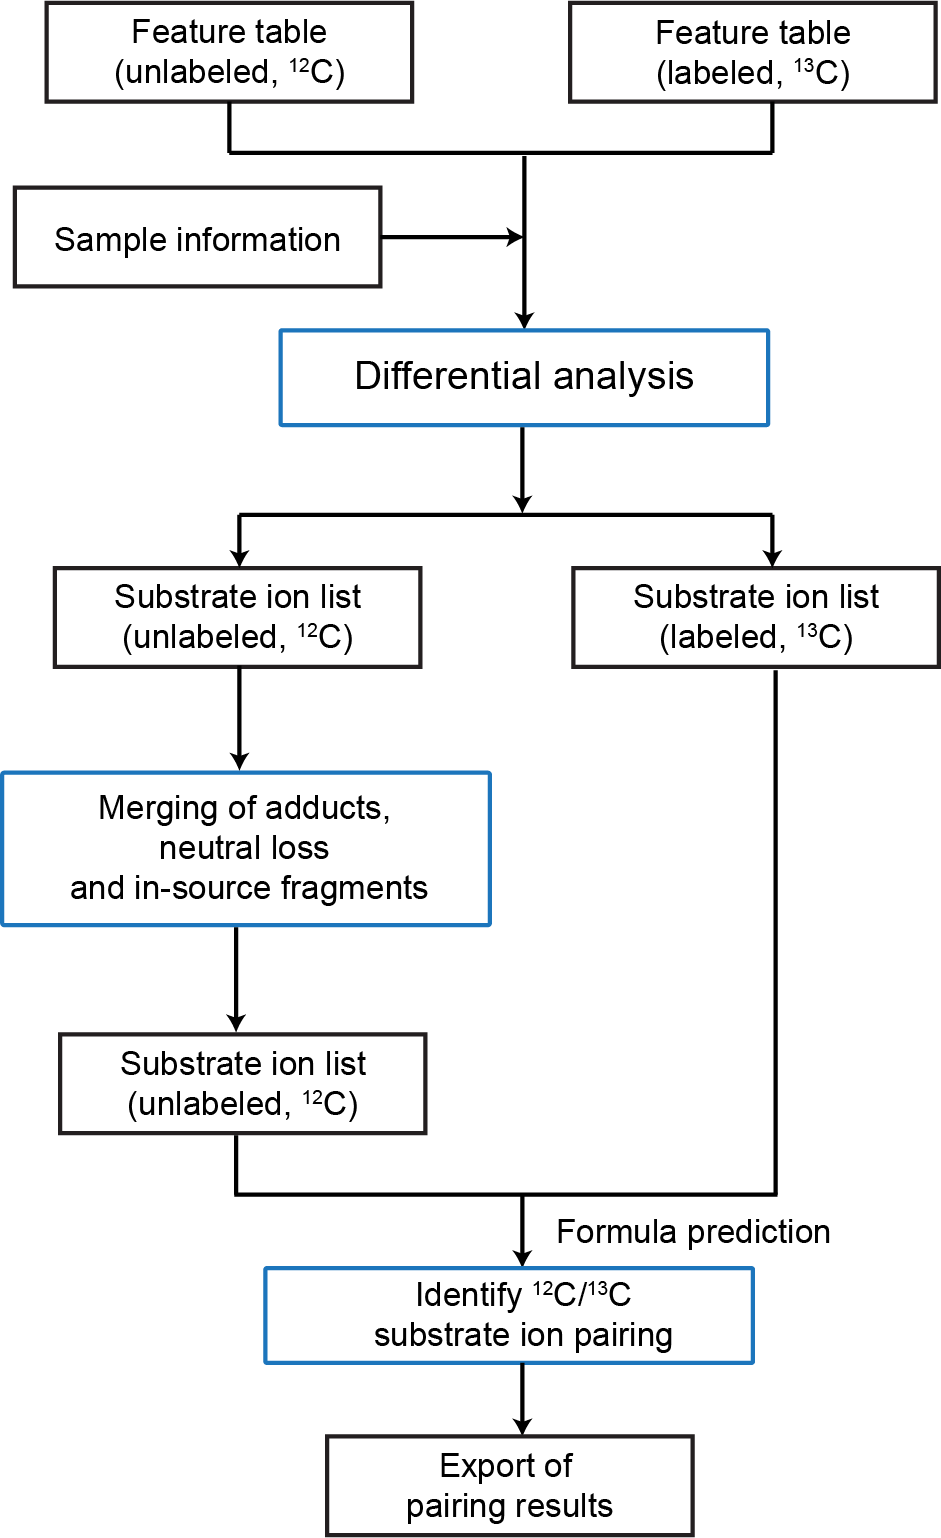
\includegraphics[width=0.5\linewidth,height=\textheight,keepaspectratio]{images/figure3_1.png}

}

\caption{\label{fig-figure3-1}Overview of the IsoPairFinder workflow.}

\end{figure}%

\section{Running IsoPairFinder and
Parameters}\label{sec-isoPairFinder-parameters}

The basic use of \texttt{IsoPairFinder} is simply running the R script
as below:

\begin{Shaded}
\begin{Highlighting}[]
\CommentTok{\# run the IsoPairFinder workflow}
\FunctionTok{library}\NormalTok{(tidyverse)}
\FunctionTok{library}\NormalTok{(IsoPairFinder)}
\CommentTok{\# analysis of HyuA}
\FunctionTok{find\_intemidates}\NormalTok{(}\AttributeTok{peak\_table\_unlabel =} \StringTok{\textquotesingle{}peak\_table\_C12.csv\textquotesingle{}}\NormalTok{,}
                 \AttributeTok{peak\_table\_label =} \StringTok{\textquotesingle{}peak\_table\_C13.csv\textquotesingle{}}\NormalTok{,}
                 \AttributeTok{sample\_info =} \StringTok{\textquotesingle{}sample\_info.xlsx\textquotesingle{}}\NormalTok{,}
                 \AttributeTok{path =} \StringTok{\textquotesingle{}\textasciitilde{}/Project/00\_Uric\_Acid\_project/Data/20250606\_isopairfind\_test/Demo\_data\_msdial/\textquotesingle{}}\NormalTok{,}
                 \AttributeTok{polarity =} \StringTok{\textquotesingle{}positive\textquotesingle{}}\NormalTok{,}
                 \AttributeTok{control\_group =} \FunctionTok{c}\NormalTok{(}\StringTok{"WT"}\NormalTok{),}
                 \AttributeTok{case\_group =} \FunctionTok{c}\NormalTok{(}\StringTok{\textquotesingle{}hyuA\textquotesingle{}}\NormalTok{),}
                 \AttributeTok{mz\_tol =} \DecValTok{10}\NormalTok{,}
                 \AttributeTok{rt\_tol =} \FloatTok{0.05}\NormalTok{,}
                 \AttributeTok{p\_value\_cutoff =} \FloatTok{0.05}\NormalTok{,}
                 \AttributeTok{p\_adjust =} \ConstantTok{TRUE}\NormalTok{,}
                 \AttributeTok{fold\_change\_cutoff =} \DecValTok{20}\NormalTok{,}
                 \AttributeTok{is\_recognize\_adducts =} \ConstantTok{TRUE}\NormalTok{)}
\end{Highlighting}
\end{Shaded}

The \texttt{find\_intemidates} function is the main function of the
IsoPairFinder package, which runs the whole workflow to identify
potential intermediates from stable isotope tracing metabolomics data.

The parameters are provided below:

\begin{itemize}
\tightlist
\item
  peak\_table\_unlabel: the feature table name of the unlabeled group.
  The default file name, ``peak\_table\_C12.csv''. See the requirements
  in Chapter~\ref{sec-data-preparation}.
\item
  peak\_table\_label: the feature table name of the unlabeled group. The
  default, ``peak\_table\_C13.csv''. See the requirements in
  Chapter~\ref{sec-data-preparation}.
\item
  sample\_info: the sample information table. See the requirements in
  Chapter~\ref{sec-data-preparation}.
\item
  path: the working path.
\item
  polarity: ionization polarity, ``positive'' or ``negative''. Default:
  ``positive''
\item
  control\_group: the control group, e.g., ``WT''. The group names
  should be included in the sample information table.
\item
  case\_group: the case group, e.g., ``hyuA''. The group names should be
  included in the sample information table.
\item
  mz\_tol: m/z tolerance (unit: ppm) for searching the intermediate
  ions. Default: 10 ppm
\item
  rt\_tol: retention time tolerance (unit: minute) for searching the
  intermediate ions. Default: 0.05 min
\item
  p\_value\_cutoff: the cutoff of p-value (t-test). Default: 0.05
\item
  p\_adjust: whether to perform the multiple comparison correction (FDR
  adjustment). Default: TRUE
\item
  fold\_change\_cutoff: the cutoff of fold-change (case vs.~control).
  Default: 20
\item
  is\_recognize\_adduct: whether to recognize and merge the isotopes,
  adducts, and in-source fragments. Default: TRUE
\end{itemize}

\section{Output}\label{sec-isoPairFinder-output}

The new folder \texttt{“00\_tracer\_result”} will be generated in the
working directory (Figure~\ref{fig-figure1-2}), including
``tracer\_pair\_result.xlsx'' and several plots in PDF files.
Specifically, these files are provided in the result folder:

\begin{itemize}
\item
  \textbf{tracer\_pair\_result.xlsx}: This file contains the results
  from differential analysis, recognized features, and identified
  substrate feature pairs. It has 4 sheets:

  \begin{itemize}
  \tightlist
  \item
    \textbf{raw\_data\_unlabeled}: the differential analysis of the
    unlabeled group. Some columns below were added to the unlabeled
    feature table, including p-values, q-values, fold changes, etc.
  \item
    \textbf{raw\_data\_labeled}: the differential analysis of the
    labeled group. Some columns below were added to the unlabeled
    feature table, including p-values, q-values, fold changes, etc.
  \item
    \textbf{recognized\_peak\_unlabel}: the table of recognized adducts,
    neutral loss, and in-source fragments (Figure~\ref{fig-figure3-2}).
    The method used here was followed from a previous
    publication\textsuperscript{6}. Some key column definitions:

    \begin{itemize}
    \tightlist
    \item
      base\_peak: the base peaks that are used to recognize the adducts
      and in-source fragments.
    \item
      relationship: the relationship with the base peak.
    \item
      num\_annotation: the number of features that belong to the same
      group.
    \item
      group\_order: the feature group ID.
    \end{itemize}
  \item
    \textbf{paired\_table}: the table of possible substrate ion pairs
    identified. Each row represents one pair of substrate ions
    (Figure~\ref{fig-figure3-2}). Specifically,

    \begin{itemize}
    \tightlist
    \item
      unlabeled\_feature\_id/mz/rt: the property (id, mz, rt) of
      substrate in the unlabeled group.
    \item
      labled\_feature\_id/mz/rt: the property (id, mz, rt) of substrate
      in the labeled group
    \item
      mass\_shift\_label: the estimated carbon number
    \item
      p\_values/fold\_changes/average\_abundance: the statistics of
      differential analysis
    \end{itemize}
  \end{itemize}
\item
  ``\textbf{volcano\_plot\_unlabeled.pdf}'' /
  ``\textbf{volcano\_plot\_labeled.pdf}'': the volcano plots that show a
  significant accumulation between the case (mutant) and control groups.
\item
  ``\textbf{isotope\_pair\_plot\_overview.pdf}'': the overview of the
  EIC mirror for identified substrate ion pairs.
\item
  ``\textbf{isotope\_pair\_list.pdf}'': the lists of EIC mirror plots
  for identified substrate ion pairs.
\item
  ``\textbf{00\_intermediate\_data}'': the intermediate data during
  processing. It was used for debugging.
\end{itemize}

\begin{figure}

\centering{

\pandocbounded{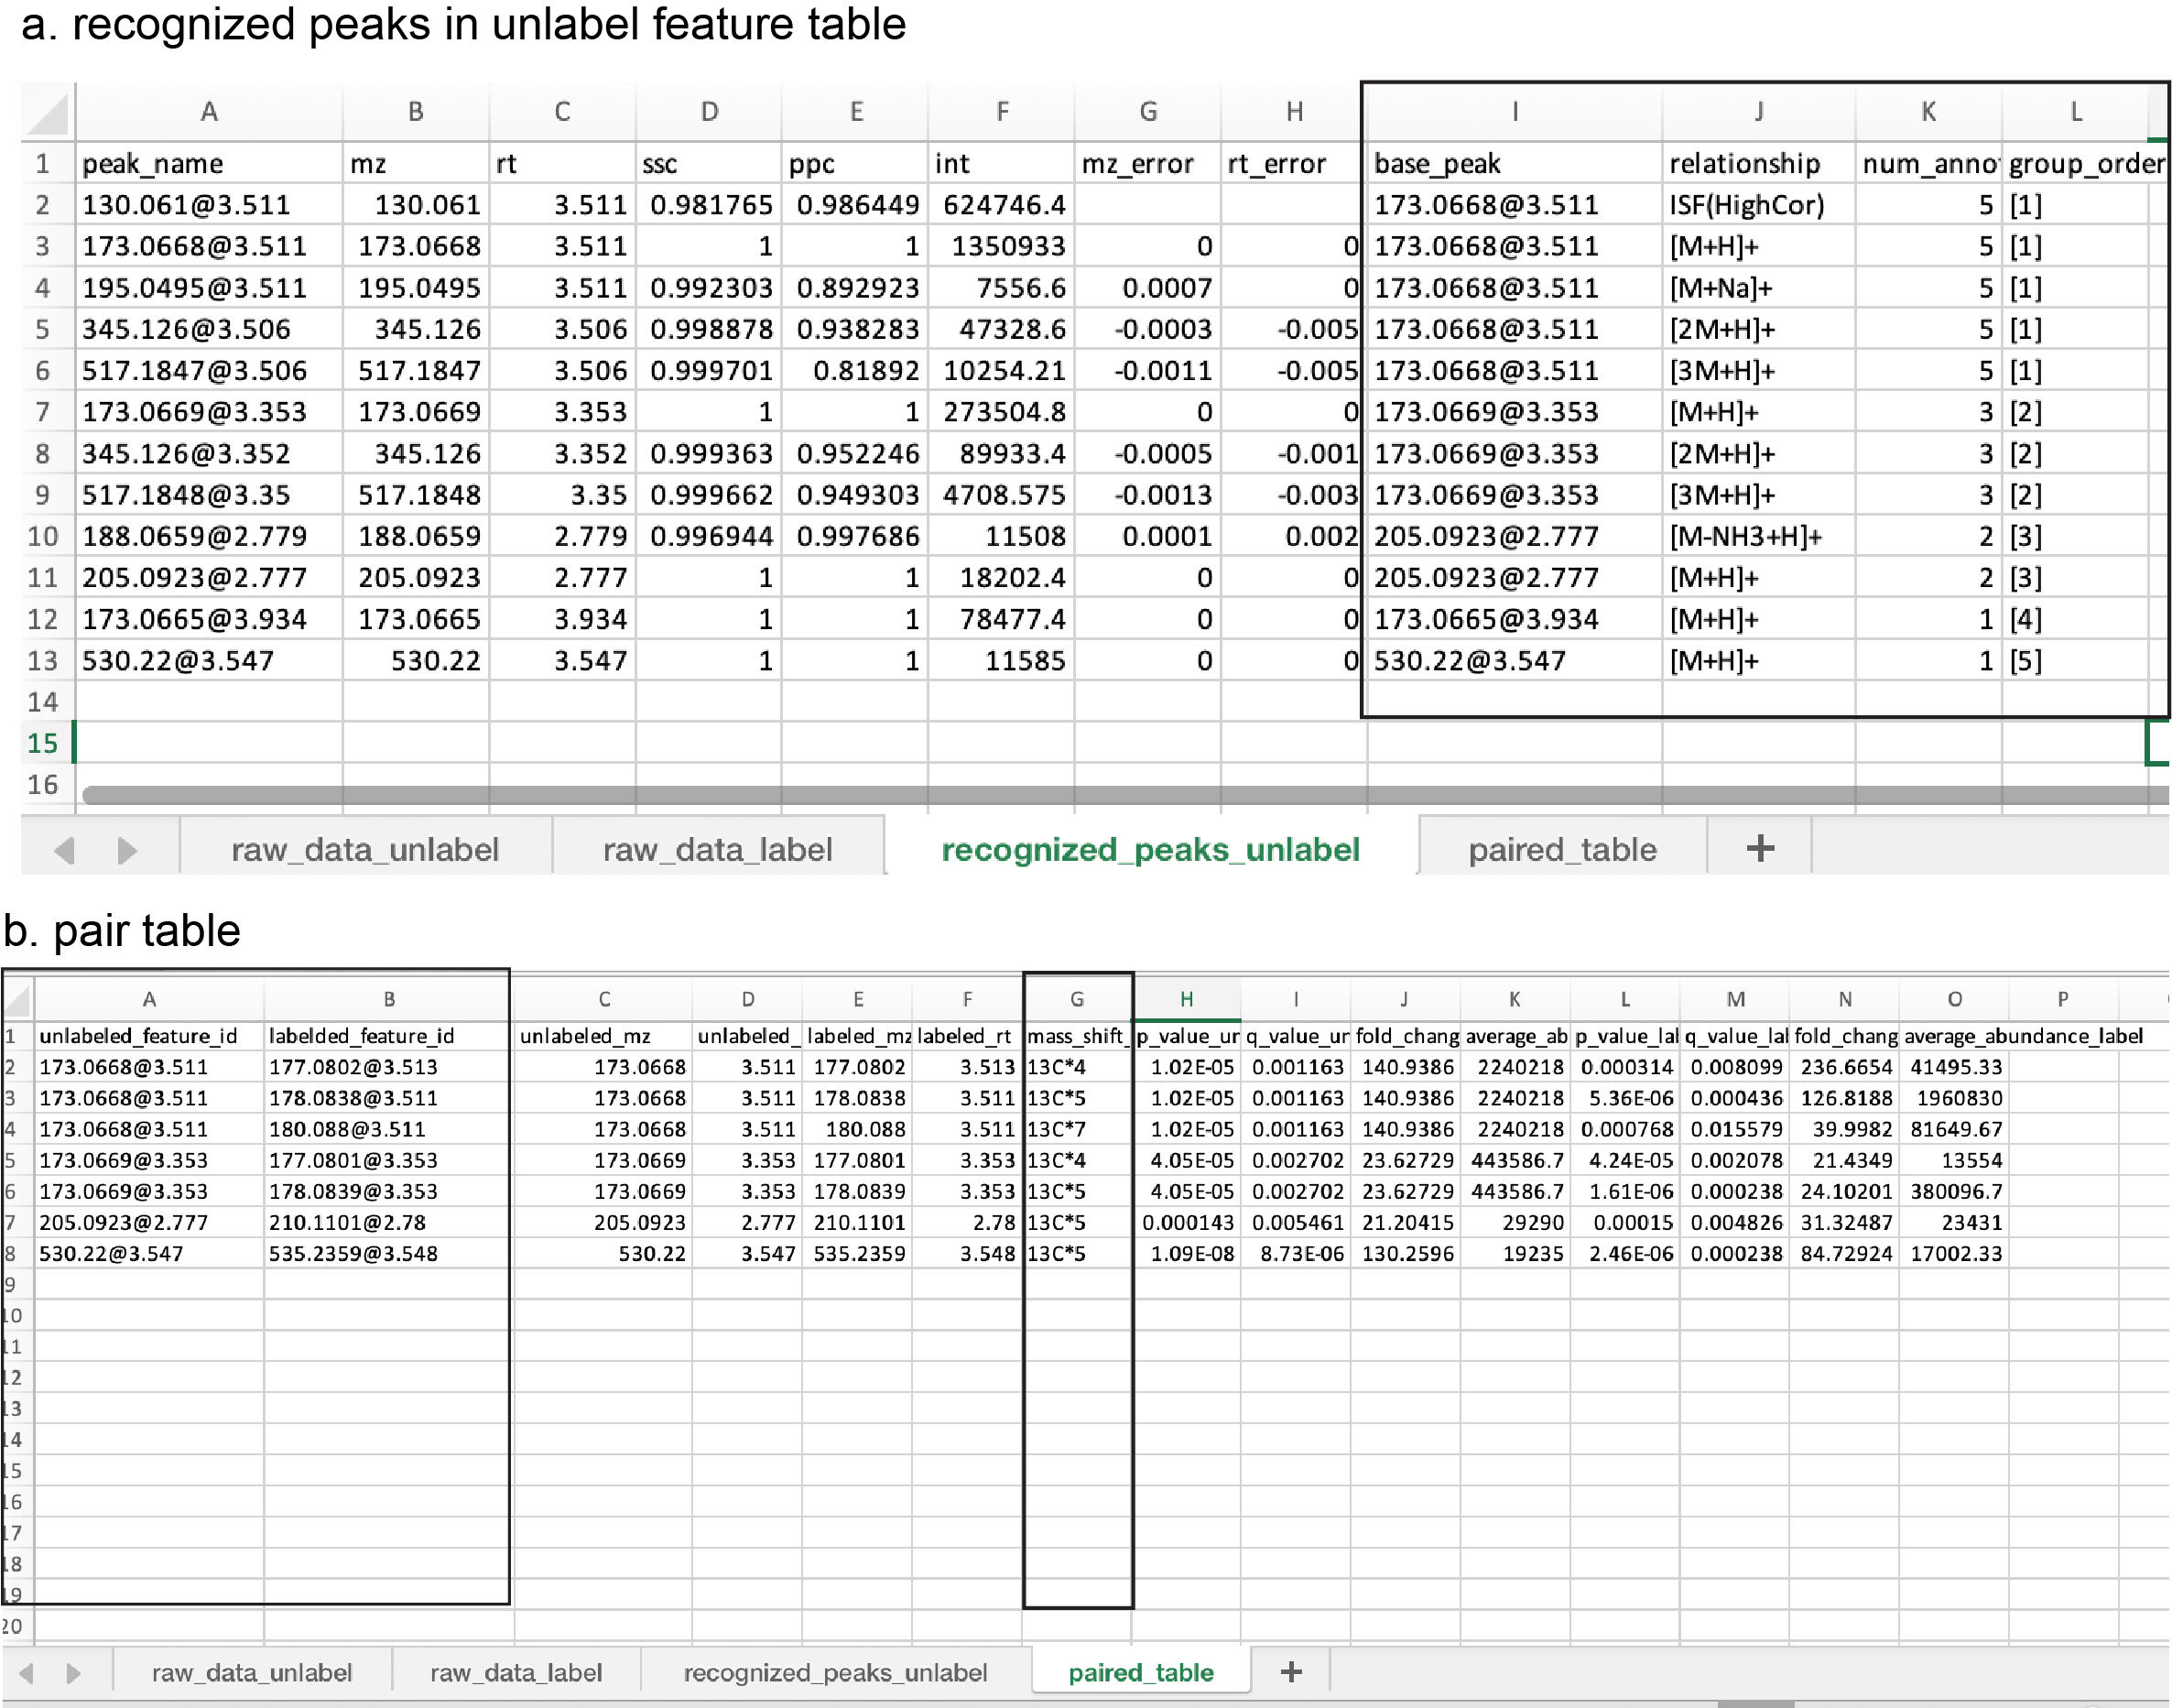
\includegraphics[keepaspectratio]{images/figure3_2.png}}

}

\caption{\label{fig-figure3-2}The screenshot of the tracer pair result
table}

\end{figure}%

\bookmarksetup{startatroot}

\chapter{Case Study}\label{sec-case-study}

The loss of uricase during hominid evolution has predisposed humans to
hyperuricemia and gout, conditions with high global prevalence. In
previous work, we identified a uric acid (UA)-inducible gene cluster in
Clostridium sporogenes that is required for converting uric acid to
short-chain fatty acids (SCFAs)\textsuperscript{1}. When these genes
were disrupted, SCFA production was blocked, yet a substantial amount of
uric acid was still consumed. This suggested the possibility that
pathway intermediates accumulate in the mutants and could be identified
by untargeted LC-MS.

To investigate this, we developed a stable isotope tracing (STI)
metabolomic experiment to detect unknown metabolites produced from uric
acid in the anaerobic mutant cultures\textsuperscript{7}. Specifically,
for the UA catabolism gene cluster, we curated the 6 mutant strains for
each gene. We cultured wild-type and mutant strains of C. sporogenes in
the presence of either unlabeled uric acid or its {[}13C5{]}-labeled
isotopologue. Here, the study of the hyuA gene was used as an example
(Figure~\ref{fig-figure4-1}).

\begin{figure}

\centering{

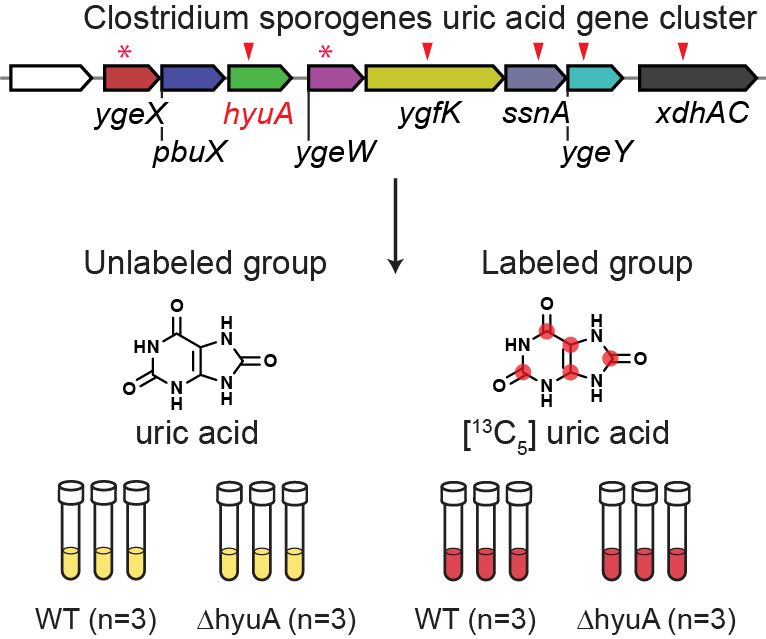
\includegraphics[width=0.5\linewidth,height=\textheight,keepaspectratio]{images/figure4_1.png}

}

\caption{\label{fig-figure4-1}Study design of STI metabolomics for
studying hyuA gene functions}

\end{figure}%

The reasonable substrate candidates have a series of characteristics:
(i) were elevated in mutant vs.~wild-type cultures, (ii) increased in
intensity over culture age, and (iii) contained retention-time matched
isotopologs when mutants were cultured with {[}13C5{]}-labeled uric
acid. We processed these STI metabolomics data using IsoPairFinder. Take
the hyuA as an example, compared to 190 possible pairs in the unlabeled
and labeled groups, IsoPairFinder could significantly narrow the
candidate pairs to 7. The final 12C/13C feature pair could be further
quickly determined, which further helps propose its possible structure
(Figure~\ref{fig-figure4-2}).

\begin{figure}

\centering{

\pandocbounded{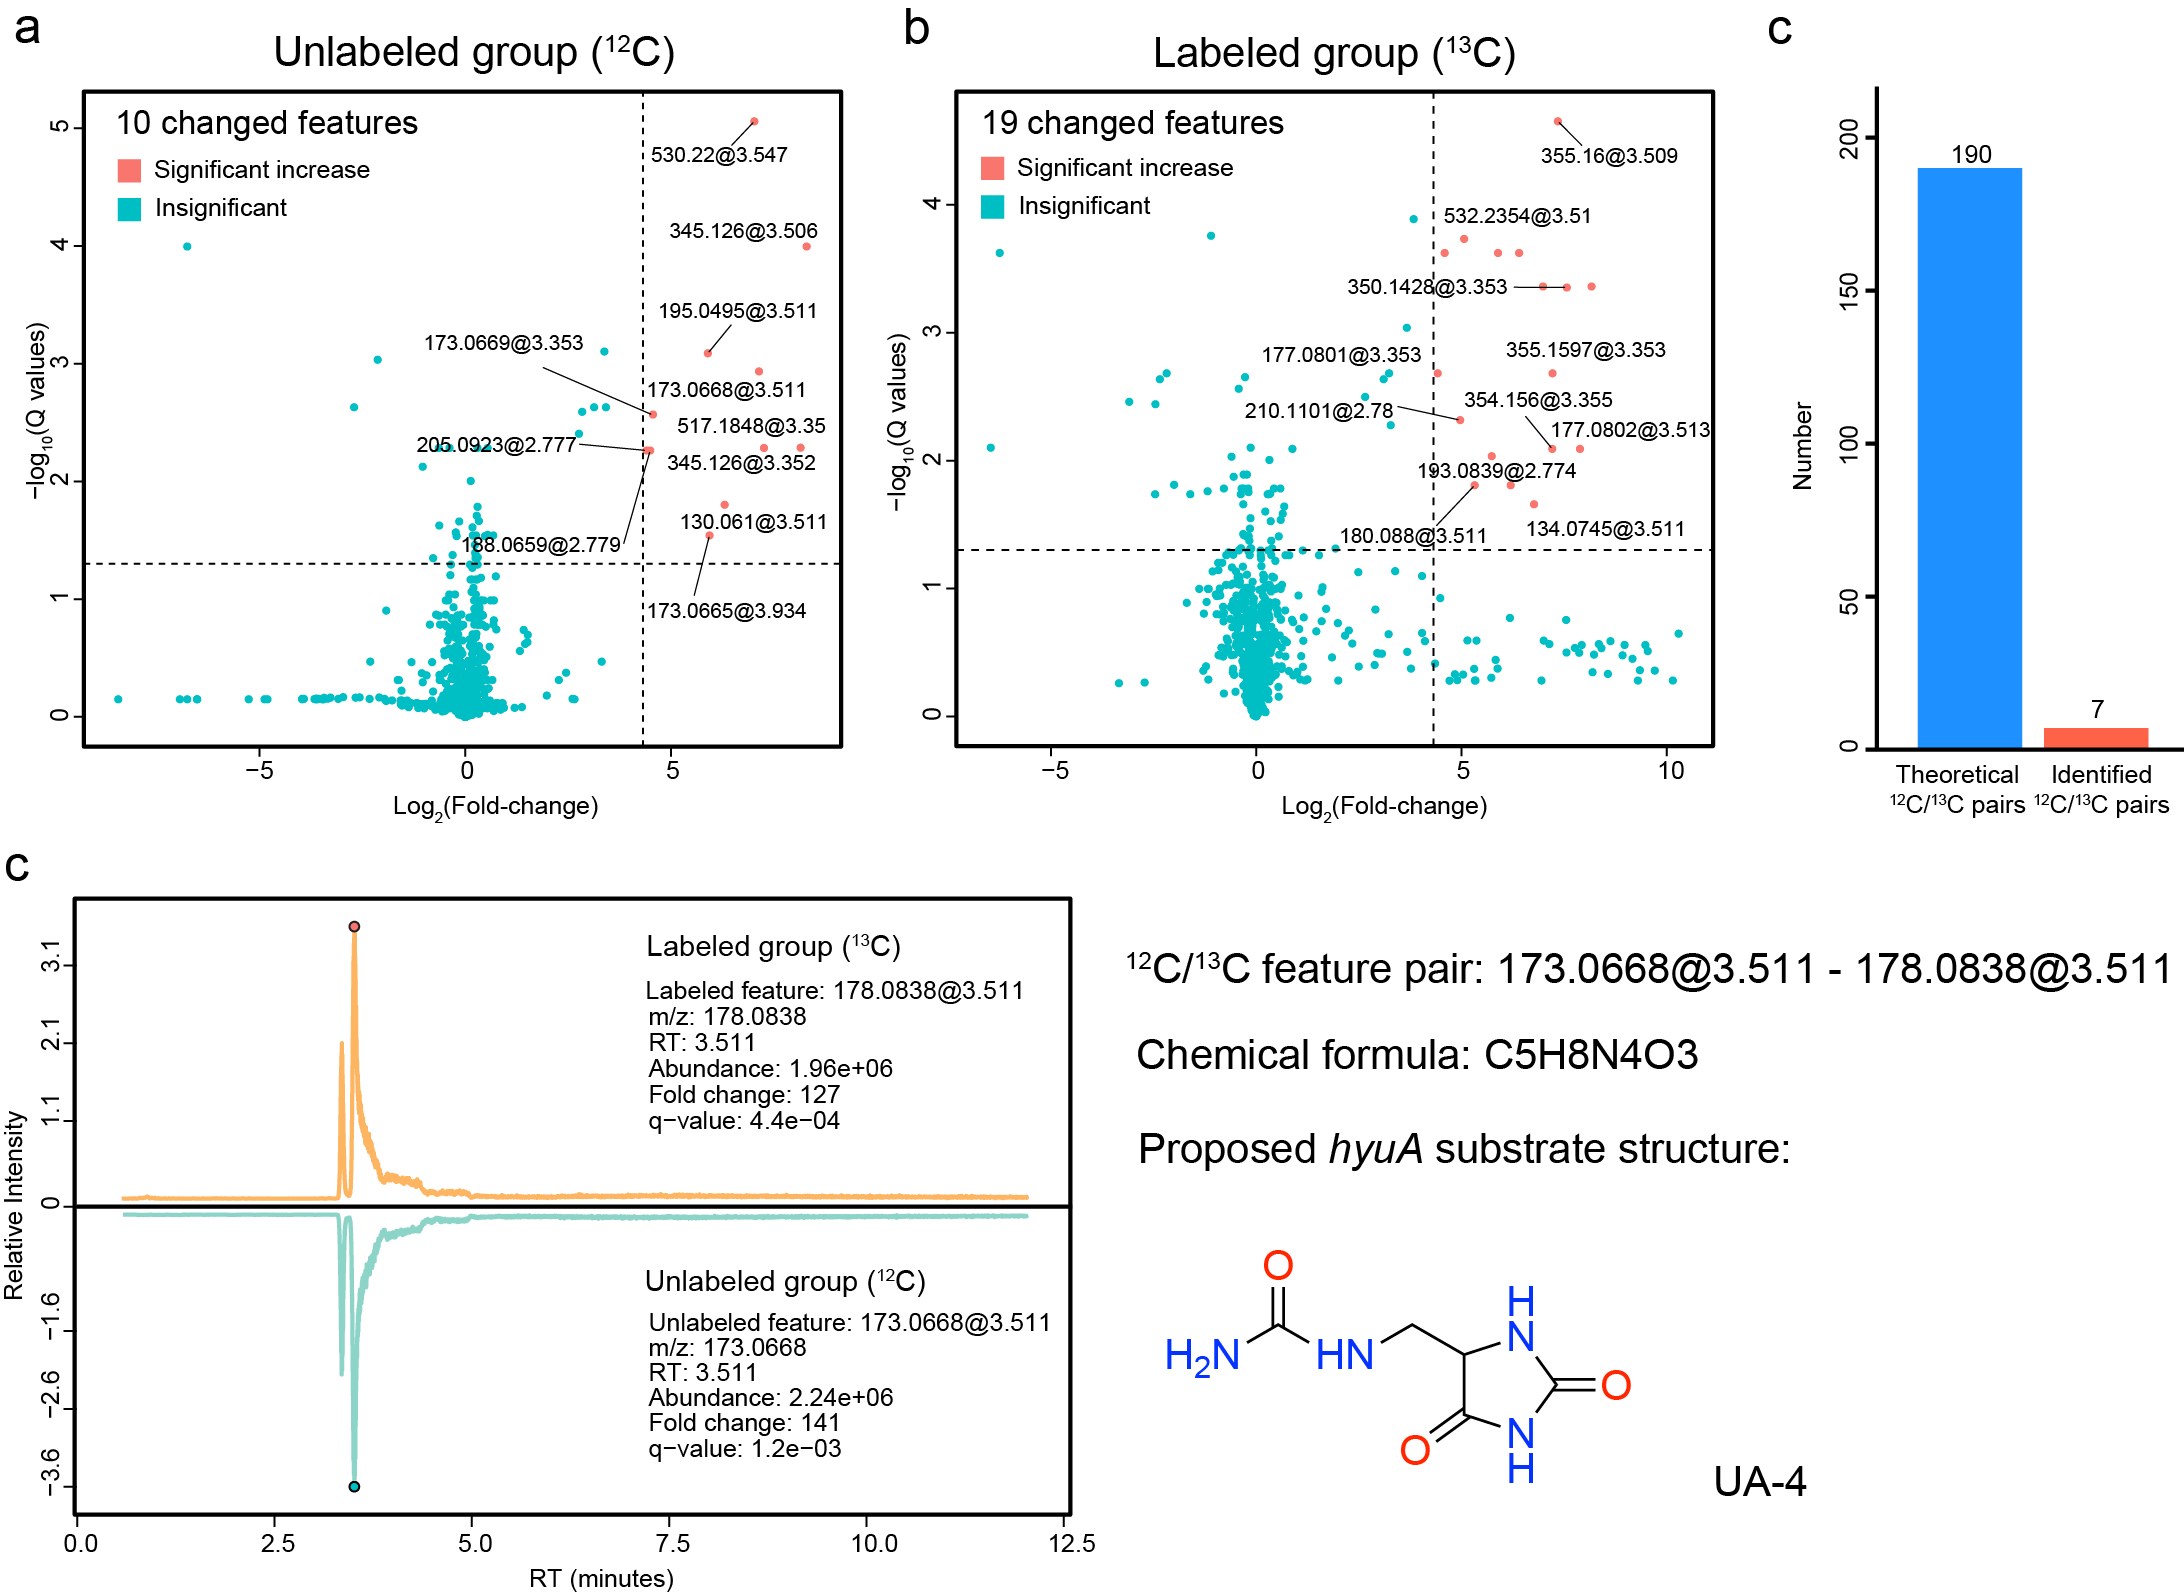
\includegraphics[keepaspectratio]{images/figure4_2.png}}

}

\caption{\label{fig-figure4-2}The identified 12C/13C feature pairs
revealing the substrate of the hyuA gene.}

\end{figure}%

\bookmarksetup{startatroot}

\chapter*{References}\label{references}
\addcontentsline{toc}{chapter}{References}

\markboth{References}{References}

\phantomsection\label{refs}
\begin{CSLReferences}{0}{0}
\bibitem[\citeproctext]{ref-liu_widely_2023}
\CSLLeftMargin{1. }%
\CSLRightInline{Liu, Y. \emph{et al.}
\href{https://doi.org/10.1016/j.cell.2023.06.010}{A widely distributed
gene cluster compensates for uricase loss in hominids}. \emph{Cell}
\textbf{186}, 3400--3413.e20 (2023).}

\bibitem[\citeproctext]{ref-smith_xcms_2006}
\CSLLeftMargin{2. }%
\CSLRightInline{Smith, C. A., Want, E. J., O'Maille, G., Abagyan, R. \&
Siuzdak, G. \href{https://doi.org/10.1021/ac051437y}{{XCMS}:
{Processing} {Mass} {Spectrometry} {Data} for {Metabolite} {Profiling}
{Using} {Nonlinear} {Peak} {Alignment}, {Matching}, and
{Identification}}. \emph{Analytical Chemistry} \textbf{78}, 779--787
(2006).}

\bibitem[\citeproctext]{ref-tsugawa_lipidome_2020}
\CSLLeftMargin{3. }%
\CSLRightInline{Tsugawa, H. \emph{et al.}
\href{https://doi.org/10.1038/s41587-020-0531-2}{A lipidome atlas in
{MS}-{DIAL} 4}. \emph{Nature Biotechnology} \textbf{38}, 1159--1163
(2020).}

\bibitem[\citeproctext]{ref-schmid_integrative_2023}
\CSLLeftMargin{4. }%
\CSLRightInline{Schmid, R. \emph{et al.}
\href{https://doi.org/10.1038/s41587-023-01690-2}{Integrative analysis
of multimodal mass spectrometry data in {MZmine} 3}. \emph{Nature
Biotechnology} \textbf{41}, 447--449 (2023).}

\bibitem[\citeproctext]{ref-kuhl_camera_2012}
\CSLLeftMargin{5. }%
\CSLRightInline{Kuhl, C., Tautenhahn, R., Böttcher, C., Larson, T. R. \&
Neumann, S. \href{https://doi.org/10.1021/ac202450g}{{CAMERA}: {An}
{Integrated} {Strategy} for {Compound} {Spectra} {Extraction} and
{Annotation} of {Liquid} {Chromatography}/{Mass} {Spectrometry} {Data}
{Sets}}. \emph{Analytical Chemistry} \textbf{84}, 283--289 (2012).}

\bibitem[\citeproctext]{ref-zhou_metabolite_2022}
\CSLLeftMargin{6. }%
\CSLRightInline{Zhou, Z. \emph{et al.}
\href{https://doi.org/10.1038/s41467-022-34537-6}{Metabolite annotation
from knowns to unknowns through knowledge-guided multi-layer metabolic
networking}. \emph{Nature Communications} \textbf{13}, 6656 (2022).}

\bibitem[\citeproctext]{ref-liu_gut_2025}
\CSLLeftMargin{7. }%
\CSLRightInline{Liu, Y. \emph{et al.}
\href{https://doi.org/10.1101/2025.04.24.650524}{Gut bacteria degrade
purines via the 2,8-dioxopurine pathway}. \emph{Nature Microbiology}
\textbf{Accepted}, (2025).}

\end{CSLReferences}




\end{document}
